\PassOptionsToPackage{main=english, polutonikogreek}{babel}
\documentclass[10pt,xcolor={dvipsnames}, aspectratio=169]{beamer}
\usetheme[]{Feather}
\usepackage{natbib}
\usepackage{graphicx}
\usepackage{tikz}
\usepackage[utf8]{inputenc}
\usepackage[english]{babel}
\usepackage{listings}
\usepackage{minted}
\usepackage{makecell}
\usepackage{amsmath, amsthm, amssymb, amsfonts}
\usepackage{tcolorbox}
\usepackage{libertine}
\usepackage{xcolor}
\usepackage{pgfplots}
\usepackage{parskip}
\usepackage{neuralnetwork}
\usepackage{xpatch}
\usepackage[T1]{fontenc}
\usepackage{zi4}
\usepackage{soul}
\usepackage{multirow, multicol}
\usepackage{academicons}
\usepackage{fontawesome}
\usepackage{pifont}
\usepackage{colortbl}
\usepackage[toc]{multitoc}
\usepackage{blindtext}
\usepackage{hologo}
\usepackage{xspace}
\usepackage{textgreek}
\usepackage[or]{teubner}
\usepackage{caption}
\usepackage{algorithm}
\usepackage{algpseudocode}

\usetikzlibrary{shapes.gates.logic.US,shapes.gates.logic.IEC}
\usetikzlibrary{automata}
\usetikzlibrary{shapes}
\usetikzlibrary{matrix,chains,positioning,decorations.pathreplacing,arrows}
\usetikzlibrary{positioning,calc}
\pgfplotsset{compat=1.18}

\newminted[ccode]{c}{frame=lines, framesep=2mm, baselinestretch=1.2, fontsize=\footnotesize, style=pastie}

\newminted[latexcode]{latex}{frame=lines, frameseo=2mm, baselinestretch=1.2, fontsize=\footnotesize, style=pastie, escapeinside=||}
\definecolor{cadetgrey}{rgb}{0.57, 0.64, 0.69}
\definecolor{latexBird}{HTML}{008080}
\definecolor{darkGreen}{HTML}{43a343}

\setbeamertemplate{itemize item}{\ding{52}}
\setbeamertemplate{caption}[numbered]
\setbeamercolor{background canvas}{bg=cadetgrey!10}
\newcommand{\tac}{\centering\arraybackslash}

\xpatchcmd{\linklayers}{\nn@lastnode}{\lastnode}{}{}
\xpatchcmd{\linklayers}{\nn@thisnode}{\thisnode}{}{}
\tikzset{%
  every neuron/.style={
    circle,
    draw,
    minimum size=1cm
  },
  neuron missing/.style={
    draw=none, 
    scale=2,
    text height=0.333cm,
    execute at begin node=\color{black}$\vdots$
  },
}
\newcommand*\circled[1]{\tikz[baseline=(char.base)]{
            \node[shape=circle,draw,inner sep=2pt] (char) {#1};}}
\tikzset{
        treenode/.style={align=center,inner sep=0pt},
        % Expanded nodes
        node_expanded/.style={treenode, circle, darkGreen, draw=darkGreen, fill=cadetgrey!10, text width=0.8cm},
        % Non-expanded nodes
        node_non_expanded/.style={treenode, circle, red, draw=red, fill=cadetgrey!10, text width=0.8cm},
        % Leaf nodes
        node_leaf/.style={treenode, rectangle, black, fill=black, minimum width=0.3cm, minimum height=0.3cm},
        % Cost nodes
        node_cost/.style={treenode, rectangle, black, dashed, draw=black, minimum width=0.5cm, minimum height=0.5cm}
}
\hypersetup{
pdftitle={Latex Workshop},
}
%-------------------------------------------------------
% INFORMATION IN THE TITLE PAGE
%-------------------------------------------------------
\title[Shiraz University]{
\includegraphics[width=0.35\textwidth]{Images/latex_long.png}}
\author{\textit{\textbf{Alireza Rostami}}}
\institute[Shiraz Universtiy]
{
	Department of Computer Science, Engineering \& IT \\
	Shiraz University
}
\date{August, 2022}

\begin{document}
\begin{frame}[plain,noframenumbering]
  \titlepage
\end{frame}

\begin{frame}{Overview}
    \begin{multicols*}{5}
        \tableofcontents
    \end{multicols*}
\end{frame}

\section{Introduction}
\begin{frame}[plain,noframenumbering]
    	\finalpage{\textcolor{Black}{\LARGE\textbf{Introduction}}}
    \end{frame}
\subsection{History}
	\begin{frame}{History}
	    \begin{columns}[T]
		    \begin{column}{0.8 \textwidth}
		    \textcolor{latexBird}{\TeX} \xspace is a \textcolor{latexBird}{typesetting system}.\\
		  \bigskip
            In the 1970s, Stanford University computer scientist \textcolor{latexBird}{Donald Knuth} was working on his book, \textit{The Art of Computer Programming}. \\
		    When he received his galley proofs back from the publisher, he realized that the then-new digital typesetting system was too poor quality for his liking. Knuth decided to come up with his own way; thus creating what would ultimately become the \TeX \xspace program.\\
            \bigskip
		    The name \TeX \xspace is a combination of the Greek capital letters \textit{tau} (\textTau), \textit{epsilon} (\textEpsilon), and \textit{chi} (\textChi). It derives from the ancient Greek word \textgreek{τέχνη} meaning skill, art, and technique.
			\end{column}
			\begin{column}{0.2 \textwidth}
			\vspace{0.5cm}
			\begin{figure}
				\begin{tikzpicture}
				\begin{scope}
					\clip [rounded corners=1cm] (0,0) rectangle coordinate (centerpoint) (3,3cm); 
					\node [inner sep=0pt] at (centerpoint)
					{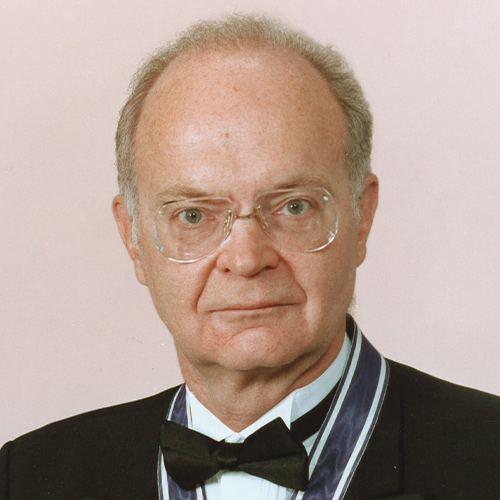
\includegraphics[width=3cm]{Images/donald_knuth.jpg}}; 
				\end{scope}
			    \end{tikzpicture}
                \captionsetup{justification=centering}
				\caption{Donald Knuth}
            \end{figure}
			\end{column}
		\end{columns}
	\end{frame}
	\begin{frame}{History}
	    \begin{columns}[T]
		    \begin{column}{0.8 \textwidth}
		    \textcolor{latexBird}{\LaTeX} \xspace is a \textcolor{latexBird}{software system} for document preparation. \\
		    \bigskip
            \LaTeX \xspace was developed in the early 1980s by  computer scientist \textcolor{latexBird}{Leslie Lamport}, when he was working at SRI. Lamport was in the process of writing his own book and found the popular macros of \TeX \xspace available at the time to be inadequate, and thought that with a little extra effort he could make a general package usable by others. \\
            \bigskip
		    The name \LaTeX \xspace is said to be an abbreviation of \textit{Lamport's \TeX}\xspace, though not verified officially.
			\end{column}
			\begin{column}{0.2 \textwidth}
			\vspace{0.5cm}
			\begin{figure}
				\begin{tikzpicture}
				\begin{scope}%[yshift=0]
					\clip [rounded corners=1cm] (0,0) rectangle coordinate (centerpoint) (3,3cm); 
					\node [inner sep=0pt] at (centerpoint)
					{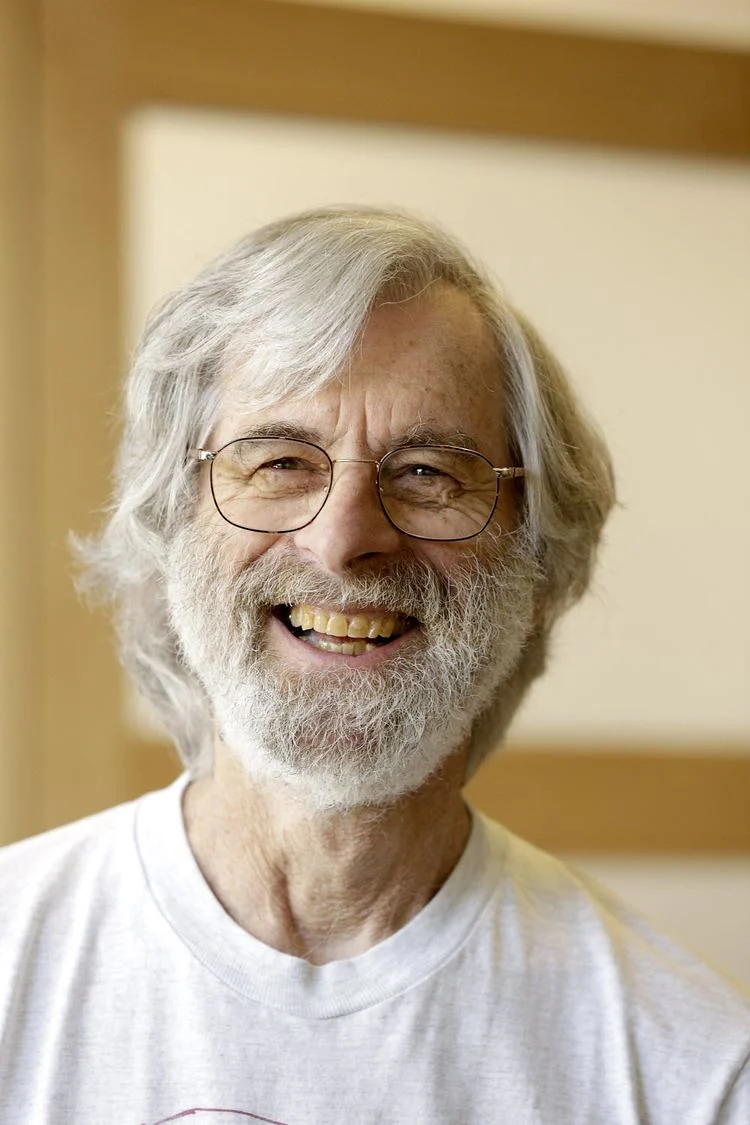
\includegraphics[width=3cm]{Images/leslie_lamport.png}}; 
				\end{scope}
			    \end{tikzpicture}
                \captionsetup{justification=centering}
				\caption{Leslie Lamport}
            \end{figure}
			\end{column}
		\end{columns}
	\end{frame}
	\subsection{Comparison}
		\begin{frame}{Comparison: Microsoft Word vs \LaTeX}
		You may be wondering why someone should use \LaTeX \xspace when we have Microsoft Word. \\ Let's compare these two.
			\begin{center}
			\begin{figure}

				\begin{tikzpicture}[line width=.1mm,rounded corners=.5em]
					\node (table) [clip,inner sep=.7\pgflinewidth] {
						\color{beamer@normaltextcolor} % text color
						\begin{tabular}[c]{|>{\tac}m{3.5cm}|>{\tac}m{5cm}|>{\tac}m{4.4cm}}
							\arrayrulecolor{beamer@headercolor}
							
							\cellcolor{beamer@headercolor}\color{white}Criterion &
							\cellcolor{beamer@headercolor}\color{white}MS Word & \cellcolor{beamer@headercolor}\color{white}\LaTeX \\ 
							
							\rowcolor{cadetgrey!30}						
							\textit{Ease of use:} & Very easy to use & Takes some time to learn \\
							
							\textit{Field of use:} & Daily use & Technical \& scientific fields \\ 
							
							\rowcolor{cadetgrey!30}							
							\textit{Price:} & Proprietary software & Free \& open-source \\
							
							\textit{Citation features:} & Difficult citation management & Easy with \hologo{BibTeX} \\ 
							
							\rowcolor{cadetgrey!30}							
							\textit{Mathematical features:} & Virtually none & Great mathematical tools \\
							
							\textit{Management:} & Difficult to change & Easy to change \\
							
							\rowcolor{cadetgrey!30}							
							\textit{Type:} & What you see is what you get & Needs to be compiled \\ 
							
							\textit{Speed with small files:} & Faster & Slower \\

							\rowcolor{cadetgrey!30}	
							\textit{Speed with large files:} & Very slow & Fast \\
							
							\textit{Compatibility:} & Not compatible with every version & Compatible (PDF output) \\
						\end{tabular}
					};
					\draw [rounded corners=.5em] (table.north west) rectangle (table.south east);
			\end{tikzpicture}
			 \captionsetup{justification=centering}
            \caption{Comparison between MS Word \& \LaTeX}
            \end{figure}
			\end{center}
 		\end{frame}
 	\subsection{Applications}
	\begin{frame}{Applications}
		\LaTeX \xspace is mostly used to write and plot mathematical and scientific formulae, graphs and plots.\\ It can also be used to write computer-science-related things like algorithms and code snippets. \\
		\medskip
		Let's see some capabilities of \LaTeX!
		\begin{figure}
		    \begin{center}
                \begin{tikzpicture}[shorten >=1pt,node distance=4cm,on grid,auto] 
                    \node[state,initial] (0)       {$Q_0$}; 
                    \node[state] (1) [above right= 3cm and 3cm of 0] {$Q_1$}; 
                    \node[state,accepting] (2) [right= 6cm of 0] {$Q_2$};
                    \path[->] 
                        (0) edge node {$\phi_{0,1}$} (1)
                            edge [bend left = 15] node {$\epsilon_{0,2}$} (2)
                        (1) edge node {$\lambda_{1,2}, \gamma_{1,2} \ $} (2)
                        (2) edge [bend left = 15] node {$\alpha_{2,0}$} (0)
                        edge [loop right] node {$\delta_{2}$} (2)
                        ;
                \end{tikzpicture}
            \end{center}
			 \captionsetup{justification=centering}
		    \caption{A simple automata}
		\end{figure}
		\end{frame}
	\begin{frame}{Applications}
	 	\begin{figure}
	 	\begin{center}
            \begin{tikzpicture}[x=1.2cm, y=1.2cm, >=stealth, scale = 0.9, transform shape]
            \foreach \m/\l [count=\y] in {1,2,3,missing,4}
                \node [every neuron/.try, neuron \m/.try] (input-\m) at (0,2.5-\y) {};
            \foreach \m [count=\y] in {1,missing,2}
              \node [every neuron/.try, neuron \m/.try ] (hidden1-\m) at (2,2-\y*1.25) {};
            \foreach \m [count=\y] in {1,missing,2}
            \node [every neuron/.try, neuron \m/.try ] (hidden1-\m) at (2,2-\y*1.25) {};
            \foreach \m [count=\y] in {1,missing,2}
              \node [every neuron/.try, neuron \m/.try ] (hidden2-\m) at (5,2-\y*1.25) {};
            \foreach \m [count=\y] in {1,missing,2}
              \node [every neuron/.try, neuron \m/.try ] (output-\m) at (7,1.5-\y) {};
              
    	    \foreach \l [count=\i] in {1,2,3,N}	
                \node at (input-\i) {$I_\l$};	
            \foreach \l [count=\i] in {1,m}	
                \node at (hidden1-\i) {$H^{(1)}_\l$};	
            \foreach \l [count=\i] in {1,m}	
                \node at (hidden2-\i) {$H^{(n)}_\l$};	
            \foreach \l [count=\i] in {1,T}	
                \node at (output-\i) {$O_\l$};
            
            \foreach \i in {1,...,4}
              \foreach \j in {1,...,2}
                \draw [->] (input-\i) -- (hidden1-\j);
            \foreach \i in {1,...,2}
              \foreach \j in {1,...,2}
                \draw [->] (hidden1-\i) -- (hidden2-\j);
            \foreach \i in {1,...,2}
              \foreach \j in {1,...,2}
                \draw [->] (hidden2-\i) -- (output-\j);
            \node [align=center, above] at (0,2) {Input\\layer};
            \node [align=center, above] at (2,2) {Hidden \\layer $1$};
            \node [align=center, above] at (5,2) {Hidden \\layer $n$};
            \node [align=center, above] at (7,2) {Output \\layer};
            \node[fill=cadetgrey!10,scale=3,inner xsep=0pt,inner ysep=5mm] at ($(hidden1-1)!.5!(hidden2-2)$) {$\dots$};
            \end{tikzpicture}
        \end{center}
        \captionsetup{justification=centering}
	 	\caption{A neural network}
	 	\end{figure}
	\end{frame}
		\begin{frame}{Applications}
	 	\begin{figure}
	 	\begin{center}
            \begin{tikzpicture}[
            ->, 
            level/.style={level distance=1.5cm},
            level 1/.style={sibling distance=5.5cm},
            level 2/.style={sibling distance=2.5cm},
            level 3/.style={sibling distance=1.25cm},
            level 4/.style={sibling distance=1.75cm, level distance=1cm},
            every node/.style={solid}, scale = 0.8, transform shape
        ]
            \node[node_expanded] {S} 
                child { node[node_expanded]{A} edge from parent [black, dashed]
                    child { node[node_expanded]{C}
                    child { node[node_leaf]{Z} }
                    edge from parent node[left]{2} }
                    child { node[node_non_expanded]{F} 
                    child { node[node_cost]{7} }
                    edge from parent node[right]{5} }
                edge from parent node[above]{2} }
                child { node[node_expanded]{B} edge from parent [black, dashed]
                    child { node[node_expanded]{D}
                        child { node[node_non_expanded]{G} 
                            child { node[node_cost]{7} }
                        edge from parent node[left]{3} }
                    edge from parent node[left]{3} }
                    child { node[node_expanded]{E} 
                        child { node[node_non_expanded]{D} 
                            child { node[node_cost]{7} }
                        edge from parent node[left]{4} }
                        child { node[node_non_expanded]{G} 
                            child { node[node_cost]{8} }
                        edge from parent node[right]{5} }
                    edge from parent node[right]{2} }
                edge from parent node[left]{1} }
                child { node[node_expanded]{C} edge from parent [cyan]
                    child { node[node_non_expanded]{D} edge from parent [black, dashed]
                    child { node[node_cost]{8} }
                    edge from parent node[left]{5} }
                    child { node[node_non_expanded]{F} edge from parent [black, dashed]
                    child { node[node_cost]{7} }
                    edge from parent node[left]{4} }
                    child { node[node_expanded]{G} edge from parent [cyan]
                    child { node[node_cost]{5} }
                    edge from parent node[right]{2} }
                edge from parent node[above]{3} }
            ;
        \end{tikzpicture}
        \end{center}
	 	\caption{A fanciful tree}
	 	\end{figure}
	\end{frame}
	\begin{frame}{Applications}
	 	\begin{figure}
	 	\begin{center}
            \begin{tikzpicture}
                \begin{axis}[
                    hide axis,
                    colormap/cool,
                ]
                \addplot3[
                   mesh,
                  samples=26,
                  domain=-6:6,
                ]
                {sin(deg(sqrt(x^2+y^2)))/sqrt(x^2+y^2)};
                \addlegendentry{\(\frac{sin(r)}{r}\)}
                \end{axis}
            \end{tikzpicture}
        \end{center}
	 	\caption{A cool 3D plot}
	 	\end{figure}
	\end{frame}
	\begin{frame}{Applications}
	 	\begin{figure}
	 	\begin{center}
            \tikzstyle{branch}=[fill,shape=circle,minimum size=3pt,inner sep=0pt]
\begin{tikzpicture}[label distance=2mm]

    \node (x3) at (0,0) {$x_3$};
    \node (x2) at (1,0) {$x_2$};
    \node (x1) at (2,0) {$x_1$};
    \node (x0) at (3,0) {$x_0$};

    \node[not gate US, draw, rotate=-90] at ($(x2)+(0.5,-1)$) (Not2) {};
    \node[not gate US, draw, rotate=-90] at ($(x1)+(0.5,-1)$) (Not1) {};
    \node[not gate US, draw, rotate=-90] at ($(x0)+(0.5,-1)$) (Not0) {};

    \node[or gate US, draw, logic gate inputs=nnn] at ($(x0)+(2,-2)$) (Or1) {};
    \node[or gate US, draw, logic gate inputs=nnnn] at ($(Or1)+(0,-1)$) (Or2) {};
    \node[or gate US, draw, logic gate inputs=nnn] at ($(Or2)+(0,-1)$) (Or3) {};
    \node[xor gate US, draw, logic gate inputs=nn] at ($(Or3)+(0,-1)$) (Xor1) {};
    \node[and gate US, draw, logic gate inputs=nn, anchor=input 1] at ($(Or3.output)+(1,0)$) (And1) {};
    \node[nor gate US, draw, logic gate inputs=nn, anchor=input 1] at ($(Or2.output -| And1.output)+(1,0)$) (Nor1) {};
    \node[and gate US, draw, logic gate inputs=nn, anchor=input 1] at ($(Or1.output -| Nor1.output)+(1,0)$) (And2) {};

    \foreach \i in {2,1,0}
    {
        \path (x\i) -- coordinate (punt\i) (x\i |- Not\i.input);
        \draw (punt\i) node[branch] {} -| (Not\i.input);
    }
    \draw (x3) |- (Or2.input 1);
    \draw (x3 |- Or1.input 1) node[branch] {} -- (Or1.input 1);
    \draw (x2) |- (Xor1.input 1);
    \draw (x2 |- Or3.input 1) node[branch] {} -- (Or3.input 1);
    \draw (Not2.output) |- (Or2.input 2);
    \draw (x1) |- (Or3.input 2);
    \draw (x1 |- Or1.input 2) node[branch] {} -- (Or1.input 2);
    \draw (Not1.output) |- (Xor1.input 2);
    \draw (Not1.output |- Or2.input 3) node[branch] {} -- (Or2.input 3);
    \draw (x0) |- (Or2.input 4);
    \draw (Not0.output) |- (Or3.input 3);
    \draw (Not0.output |- Or1.input 3) node[branch] {} -- (Or1.input 3);
    \draw (Or3.output) -- (And1.input 1);
    \draw (Xor1.output) -- ([xshift=0.5cm]Xor1.output) |- (And1.input 2);
    \draw (Or2.output) -- (Nor1.input 1);
    \draw (And1.output) -- ([xshift=0.5cm]And1.output) |- (Nor1.input 2);
    \draw (Or1.output) -- (And2.input 1);
    \draw (Nor1.output) -- ([xshift=0.5cm]Nor1.output) |- (And2.input 2);
    \draw (And2.output) -- ([xshift=0.5cm]And2.output) node[above] {$f_1$};

\end{tikzpicture}

        \end{center}
	 	\caption{A logical circuit}
	 	\end{figure}
	\end{frame}
	\begin{frame}[fragile]{Applications}
		\begin{columns}[T]
        \begin{column}{0.5 \textwidth}
        \begin{figure}
	 	\begin{center}
	 	\begin{algorithm}[H]
        \caption{Power}
        \begin{algorithmic}
\smallskip
\Require $n \geq 0$
\Ensure $y = x^n$
\State $y \gets 1$, \State $X \gets x$, \State $N \gets n$
\While{$N \neq 0$}
    \State $y \gets y \times X$
    \State $N \gets N - 1$
\EndWhile
\smallskip
        \end{algorithmic}
        \end{algorithm}
        \end{center}
	 	\caption{An algorithm}
	 	\end{figure}
        \end{column}
        \begin{column}{0.5 \textwidth}
        \begin{figure}
            \centering
            \vspace{0.9cm}
                        \begin{ccode}
int power(int x, int n) {
    int X = x;
    int N = n;
    int y = 1;
    while (N != 0) {
        y *= X;
        N -= 1;
    }
    return y;
}
            \end{ccode}
            \caption{A C code snippet}
        \end{figure}
        \end{column}
        \end{columns}
    \end{frame}
	\begin{frame}{Applications}
	    None of those figures were pictures! All of them were created at compile-time by \LaTeX. None of those figures can be implemented using something like MS Word.
	    
	    \LaTeX \xspace can also be used to make presentation slides with \textcolor{latexBird}{Beamer}, like this one I am using right now.
	    
	    Thus far, I hope I have convinced you why \LaTeX \xspace is an absolute beast for technical fields. Now, let's get started with \LaTeX!
    \end{frame}
    \subsection{Getting started}
    \begin{frame}{How to use \LaTeX?}
        \TeX \xspace has a lot of engines and \LaTeX \xspace a lot of compilers. There are also a lot of platforms for working with \LaTeX \xspace, both online and offline.
        \setbeamertemplate{itemize items}[circle]
        \begin{itemize}
            \item Online
            \begin{itemize}
                \item \textbf{Overleaf (recommended)}
                \item Texlive
                \item Tutorialspoint
            \end{itemize}
            \item Offline
                \begin{itemize}
                    \item WinEdt with MiKTeX
                    \item Texstudio with Tex Live
                \end{itemize}
        \end{itemize}
        In this workshop, we use \textit{Overleaf} platform with \hologo{pdfLaTeX} as our compiler.
    \end{frame}
        \begin{frame}{Are there any differences between different compilers?}
        Yes, they are out of scope of this workshop.
        If you are interested, you can look up \href{https://www.overleaf.com/learn/latex/Choosing_a_LaTeX_Compiler}{\color{latexBird}{\underline{this link}}} from Overleaf official website and \href{https://tex.stackexchange.com/questions/13593/the-differences-between-tex-engines}{\color{latexBird}{\underline{this link}}} from Stackexchange. \\
        \medskip
        They explain the differences in detail.
    \end{frame}

\begin{frame}{Setting up Overleaf}
    Let's setup an account on Overleaf and make a quick introduction to its features.
    \bigskip
    \begin{center}
    \begin{columns}
        \begin{column}{0.5 \textwidth}
        \begin{block}{Live!}
			Let's do it live!
		\end{block}
		\end{column}
    \end{columns}
    \end{center}
\end{frame}

\section{Document structure}
\begin{frame}[plain,noframenumbering]
    \finalpage{\textcolor{Black}{\LARGE\textbf{Document Structure}}}
\end{frame}
\subsection{Structure of \LaTeX \xspace files}
    \begin{frame}[fragile]{Structure of \LaTeX \xspace files}
    The overall structure of a \LaTeX \xspace is as follows:
    \smallskip
    \begin{columns}
        \begin{column}{0.9 \textwidth}
        \begin{minted}[baselinestretch=1.2, fontsize=\footnotesize, style=pastie, escapeinside=||,]{latex}
\documentclass[options]{class}
\usepackage{packages}
\begin{document||}
    ...
\end{document||}
    \end{minted}
		\end{column}
    \end{columns}
    \smallskip
    The typical classes are the following:
    \begin{center}
    \begin{columns}
        \begin{column}{0.52 \textwidth}
        \begin{block}{Classes}
			article, standalone, report, book, letter, beamer, ...
		\end{block}
		\end{column}
    \end{columns}
    \end{center}
    The full list of classes is noted in \href{https://ctan.org/topic/class}{\color{latexBird}{\underline{this link}}}, if you are interested.
\end{frame}
\begin{frame}[fragile]{Structure of \LaTeX \xspace files - Example}
    Here's an example, with a approximation of what the output looks like.
    \smallskip
    \begin{columns}
        \begin{column}{0.5 \textwidth}
        \begin{minted}[baselinestretch=1.2, fontsize=\footnotesize, style=pastie, escapeinside=||,]{latex}
\documentclass[12pt]{article}
\usepackage{tabularx, graphics, tikz, xspace}
\begin{document||}
    Hello math! \\
    This is my first \LaTeX \xspace program! \\
    Let's write a formula:
    $$ e^{i\pi} + 1 = 0 $$
\end{document||}
    \end{minted}
		\end{column}
		\begin{column}{0.5 \textwidth}
		\begin{block}{Output}
			Hello math! \\
            This is my first \LaTeX \xspace program! \\
            Let's write a formula:
            $$ e^{i\pi} + 1 = 0 $$
		\end{block}
		\end{column}
    \end{columns}
    \bigskip
    \begin{center}
    \begin{columns}
        \begin{column}{0.5 \textwidth}
        \begin{block}{Live!}
            Let's see the exact output of this code snippet \textcolor{latexBird}{live}!
		\end{block}
		\end{column}
    \end{columns}
    \end{center}
\end{frame}
\subsection{Document Information}
\begin{frame}[fragile]{Document Information}
    In \LaTeX, we can easily specify the information of the document we have.
    \smallskip
    \begin{columns}
        \begin{column}{0.9 \textwidth}
        \begin{minted}[baselinestretch=1.2, fontsize=\footnotesize, style=pastie, escapeinside=||,]{latex}
        
\documentclass{article}
\usepackage{tabularx, graphics, tikz, xspace}
\title{\LaTeX \xspace is awesome!}
\author{Alireza Rostami}
\date{\today}
\begin{document||}
    \maketitle
\end{document||}    

        \end{minted}
		\end{column}
    \end{columns}
    \bigskip
    \begin{center}
    \begin{columns}
        \begin{column}{0.5 \textwidth}
        \begin{block}{Live!}
            Let's see the exact output of this code snippet \textcolor{latexBird}{live}!
		\end{block}
		\end{column}
    \end{columns}
    \end{center}
\end{frame}

\begin{frame}[fragile]{Document Information - Continued}
    With the help of some packages, we can even include more information entries.
    \smallskip
    \begin{columns}
        \begin{column}{0.9 \textwidth}
        \begin{minted}[baselinestretch=1.2, fontsize=\footnotesize, style=pastie, escapeinside=||,]{latex}
        
\documentclass{article}
\usepackage{xspace, authblk}
\title{\LaTeX \xspace is awesome!}
\author{Alireza Rostami%
  \thanks{Email: \texttt{ali.r.rostami79@gmail.com}}}
\affil{Department of Computer Science, Engineering \& IT, \\ Shiraz University}
\author{John Doe%
  \thanks{Email: \texttt{doe@math.nowhereu.edu}}}
\affil{Department of Mathematics, University of Nowhere}
\date{\today}
\begin{document||} \maketitle \end{document||}
        \end{minted}
		\end{column}
    \end{columns}
    \begin{center}
    \begin{columns}
        \begin{column}{0.5 \textwidth}
        \begin{block}{Live!}
            Let's see the exact output of this code snippet \textcolor{latexBird}{live}!
		\end{block}
		\end{column}
    \end{columns}
    \end{center}
\end{frame}
\subsection{Sections and chapters}
\begin{frame}[fragile]{Sections and chapters}
    Documents usually have some form of “logical structure”: division into chapters, sections, sub-sections, etc. to organize their content. \LaTeX \xspace supports the creation of a document structure and also enables customization of sectioning and numbering. The commands available to organize a document depend on the document class being used, although the simplest form of organization, sectioning, is available in all formats.
    \end{frame}
    
    \begin{frame}[fragile]{Sections and chapters}
    Let’s begin with a basic example to demonstrate the\mintinline{latex}{\section{section title}} command, which marks the beginning of a new section called section title. Section numbering is automatic and can be customized, or disabled.

    \smallskip
    \begin{columns}
        \begin{column}{0.5 \textwidth}
        \begin{minted}[baselinestretch=1.2, fontsize=\footnotesize, style=pastie, escapeinside=||,]{latex}
        
\documentclass{article}
\title{Sections and Chapters}
\author{semp\_fi}
\date{\today}
\begin{document}
    \maketitle
    \section||{Introduction}
    This is the first section.
    \section||{Second Section}
    This is the second section
\end{document}
        \end{minted}
		\end{column}
		\begin{column}{0.3 \textwidth}
        \begin{block}{Live!}
            Let's see the exact output of this code snippet \textcolor{latexBird}{live}!
		\end{block}
		\end{column}
    \end{columns}
\end{frame}
\begin{frame}[fragile]{Sections and chapters}
    LaTeX can organize, number, and index chapters and sections of document. There are up to 7 levels of depth for defining sections depending on the document class.
    
    Usually, \mintinline{latex}{\section} is the top-level document command in most documents. However, in reports or books, and similar long documents, this would be \mintinline{latex}{\chapter} or \mintinline{latex}{\part}.
    \begin{center}
        \begin{tabular}{|c|l|}
                \hline
                \thead{\textbf{Level}} & 
                \thead{\textbf{Command}}  \\
                \hline
                \textit{-1} & \mintinline{latex}{\part{part}} \\
                \textit{0} & \mintinline{latex}{\chapter{chapter}} \\
                \textit{1} & \mintinline{latex}{\section{section}} \\
                \textit{2} & \mintinline{latex}{\subsection{subsection}} \\
                \textit{3} & \mintinline{latex}{\subsubsection{subsubsection}} \\
                \textit{4} & \mintinline{latex}{\paragraph{paragraph}} \\
                \textit{5} & \mintinline{latex}{\subparagraph{subparagraph}} \\
                \hline
            \end{tabular}
    \end{center}
\end{frame}

\begin{frame}[fragile]{Unnumbered sections}
    To get an unnumbered chapter, section, subsection, etc. add an asterisk (*) at the end of the command, before the opening curly brace. These will not go into the table of contents. Here is our first example (above) but this time using \mintinline{latex}{\section*} instead of \mintinline{latex}{\section}:
    
    \smallskip
    \begin{columns}
        \begin{column}{0.5 \textwidth}
        \begin{minted}[baselinestretch=1.2, fontsize=\footnotesize, style=pastie, escapeinside=||,]{latex}
        
\documentclass{article}
\title{Unnumbered sections}
\author{semp\_fi}
\date{\today}
\begin{document}
    \maketitle
    \section||{Introduction}
    This is the first section.
    \section*||{Second Section}
    This is the second section (unnumbered).
\end{document}
        \end{minted}
		\end{column}
		\begin{column}{0.3 \textwidth}
        \begin{block}{Live!}
            Let's see the exact output of this code snippet \textcolor{latexBird}{live}!
		\end{block}
		\end{column}
    \end{columns}
\end{frame}
\begin{frame}[fragile]{Unnumbered sections - Continued}
    To add an unnumbered section to the table of contents, use the \mintinline{latex}{\addcontentsline{toc}{section}{Title of the section}} command.
    
    Here's an example:
    \begin{columns}
        \begin{column}{0.5 \textwidth}
        \begin{minted}[baselinestretch=1.2, fontsize=\footnotesize, style=pastie, escapeinside=||,]{latex}
        
\documentclass{article}
\title{Unnumbered section in table of contents} \author{semp\_fi}
\begin{document}
    \maketitle
    \tableofcontents
    \section||{Introduction}
    This is the first section (numbered).
    \addcontentsline{toc}{section}{Unnumbered Section}
    \section*||{Unnumbered Section}
    An unnumbered section.
    \section||{Second section}
    The second numbered section.
\end{document}
        \end{minted}
		\end{column}
		\begin{column}{0.3 \textwidth}
        \begin{block}{Live!}
            Let's see the exact output of this code snippet \textcolor{latexBird}{live}!
		\end{block}
		\end{column}
    \end{columns}
\end{frame}
\begin{frame}[fragile]{Section - Challenge}
    Here's three quizzes for you. You are encouraged to search the Internet to get the answers.
    \medskip
    \begin{block}{Quiz 1}
        How to change the section number from Arabic numerals to Roman numerals?
	\end{block}
	\medskip
	\begin{block}{Quiz 2}
        How to hide the section number in subsection?
	\end{block}
	\medskip
	\begin{block}{Quiz 3}
        How to get a subsubsection like this?
        2. b. iii
	\end{block}
\end{frame}

\subsection{Table of contents}
\begin{frame}[fragile]{Table of contents}
    To create the table of contents is straightforward, the command  \mintinline{latex}{\tableofcontents} does\\ the job, as seen before. The default title for the table of contents is "Contents", this can be changed into whatever you need.

    Here's an example:
    \begin{columns}
        \begin{column}{0.5 \textwidth}
        \begin{minted}[baselinestretch=1.2, fontsize=\footnotesize, style=pastie, escapeinside=||,]{latex}
        
\documentclass{article}
\title{Sections and Chapters} \author{semp\_fi} \date{ }
\renewcommand*\contentsname{Summary}
\begin{document}
    \maketitle \tableofcontents
    \section||{Introduction}
    This is the first section.
    \section||{Second Section}
    This is the second section.    
    \section||{Third Section}
    This is the third section.
\end{document}
        \end{minted}
		\end{column}
		\begin{column}{0.3 \textwidth}
        \begin{block}{Live!}
            Let's see the exact output of this code snippet \textcolor{latexBird}{live}!
		\end{block}
		\end{column}
    \end{columns}
\end{frame}

\section{Formatting}
\begin{frame}[plain,noframenumbering]
    \finalpage{\textcolor{Black}{\LARGE\textbf{Formatting}}}
\end{frame}

\subsection{Line breaks \& blank spaces}
\begin{frame}[fragile]{Line breaks}
    The most standard way how to break lines is to create a new paragraph. This is done by leaving an empty line in the code.
    
    Here's an example:
    \begin{columns}
        \begin{column}{0.5 \textwidth}
        \begin{minted}[baselinestretch=1.2, fontsize=\footnotesize, style=pastie, escapeinside=||,]{latex}
        
\documentclass{article}
\begin{document}
    Here's a demonstration.
    As you can see,
    single line
    break in the code
    acts as a space in text.
    
    However, leaving an empty line starts a new paragraph.
\end{document}

        \end{minted}
		\end{column}
		\begin{column}{0.45 \textwidth}
		\vspace{-2cm}
        \begin{block}{Result}
    Here's a demonstration.
    As you can see,
    single line
    break in the code
    acts as a space in text.
    
    However, leaving an empty line starts a new paragraph.
		\end{block}
		\end{column}
    \end{columns}
\end{frame}
\begin{frame}[fragile]{Line breaks - Continued}
    There's more than one way to insert line breaks.
    \setbeamertemplate{itemize items}[circle]
    \setlength\itemsep{0.5mm}
    \begin{itemize}
        \item \mintinline{latex}{\\}
        \item \mintinline{latex}{\newline}
    \end{itemize}
    There are additional line-breaking commands, though not used very often.
        \begin{center}
        \scalebox{0.8}[0.7]{%

        \begin{tabular}{|c|l|}
                \hline
                \thead{\textbf{Command}} & 
                \thead{\textbf{Description}}  \\
                \hline
                \mintinline{latex}{\\*} & \makecell[l]{breaks the line at the point of the command \\ and additionally prohibits a page break after the forced line break.} \\
                                \hline
                \mintinline{latex}{\break} & \makecell[l]{breaks the line without filling the current line.\\ This will result in very bad formatting if you do not fill the line yourself.} \\
                                \hline

                \mintinline{latex}{\hfill \break} & \makecell[l]{This will produce the same result as \mintinline{latex}{\newline} and \mintinline{latex}{\\}.} \\
                \hline
                \mintinline{latex}{\linebreak[number]} & \makecell[l]{breaks the line at the point of the command.\\ The number provided as an argument represents \\ the priority of the command in a range of 0 to 4. \\(0 means it will be easily ignored and 4 means do it anyway).\\ When this line break option is used, \\ \LaTeX \xspace will try to produce the best line breaks possible.} \\
                                \hline
            \end{tabular}
        }
    \end{center}
 \end{frame}
\begin{frame}[fragile]{Line breaks - Continued}
   
    Here's an example:
    \begin{columns}
        \begin{column}{0.5 \textwidth}
        \begin{minted}[baselinestretch=1.2, fontsize=\footnotesize, style=pastie, escapeinside=||,]{latex}
        
\documentclass{article}
\usepackage[utf8]{inputenc}

\begin{document}
    Something in this document. This paragraph contains no information 
    and its purposes is to provide an example on how to insert white 
    spaces and lines breaks. \\
    When a line break is inserted, the text is not indented, there 
    are a couple of extra commands do line breaks. \newline
    This paragraph provides no information whatsoever. We are exploring 
    line breaks. \hfill \break
    See the results.
\end{document}

        \end{minted}
		\end{column}
		\begin{column}{0.3 \textwidth}
		\vspace{-5cm}
        \begin{block}{Live!}
            Let's see the exact output of this code snippet \textcolor{latexBird}{live}!
		\end{block}
		\end{column}
    \end{columns}
\end{frame}

\begin{frame}[fragile]{Page breaks}
   There are three commands to insert page breaks, \mintinline{latex}{\clearpage}, \mintinline{latex}{\newpage} and \mintinline{latex}{\pagebreak}.
    
    If the command \mintinline{latex}{\clearpage} is used, and there are stacked floating elements, such as tables or figures, they will be flushed out before starting the new page. If the page break is inserted before all the figures are displayed, remaining images are inserted in an empty page before continuing with the text below the break point. We mostly do not use \mintinline{latex}{\clearpage}.

    Command \mintinline{latex}{\newpage} and \mintinline{latex}{\pagebreak} are analogous to \mintinline{latex}{\newline} and \mintinline{latex}{\linebreak} respectively. 
\end{frame}

\begin{frame}[fragile]{Page breaks - Continued}
   The difference bewteen \mintinline{latex}{\pagebreak} and \mintinline{latex}{\newline} is shown by the below figure.
   	\begin{figure}
		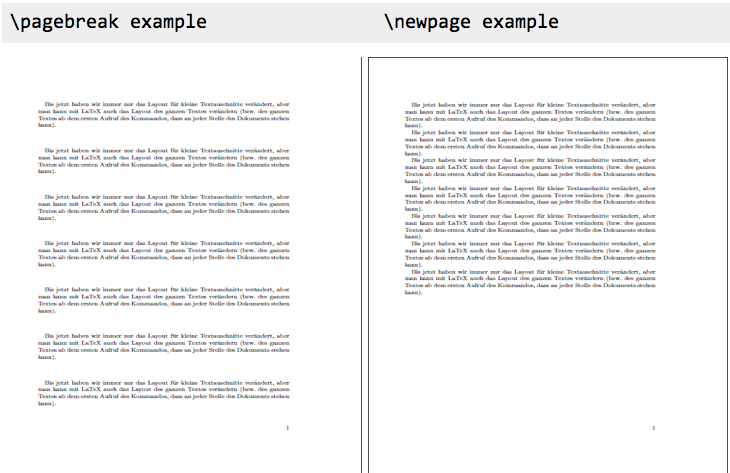
\includegraphics[width=8.5cm]{Examples/pagebreak_newpage.png}; 
        \captionsetup{justification=centering}
		\caption{Difference Between \mintinline{latex}{\pagebreak} and \mintinline{latex}{\newpage}}
    \end{figure}
\end{frame}

\begin{frame}[fragile]{Horizontal blank spaces}
    There are two commands that insert horizontal blank spaces:
    \setbeamertemplate{itemize items}[circle]
    \setlength\itemsep{0.5mm}
    \begin{itemize}
        \item \mintinline{latex}{\hspace{num}}: \\ \hspace{1.2em} Inserts a horizontal space of length $ num $. Other \LaTeX \xspace units can be used with this command. Horizontal spaces of arbitrary length may be inserted with this command.

        \item \mintinline{latex}{\hfill}: \\ \hspace{1.2em} Inserts a blank space that will stretch accordingly to fill the space available.
        The commands \mintinline{latex}{\hrulefill} and \mintinline{latex}{\dotfill} do the same as \mintinline{latex}{\hfill} but instead of blank spaces they insert a horizontal ruler and a string of dots, respectively.
    \end{itemize}
\end{frame}

\begin{frame}[fragile]{Horizontal blank spaces - Example}
        \begin{columns}
        \begin{column}{0.7 \textwidth}
        \begin{minted}[baselinestretch=1.2, fontsize=\footnotesize, style=pastie, escapeinside=||,]{latex}
        
\documentclass{article}
\usepackage[utf8]{inputenc}

\begin{document}
    Horizontal \hspace{1cm} spaces can be inserted manually. 
    Useful to control the fine-tuning in the layout of pictures.
    
    Left Side \hfill Right Side \\
    Left Side \hrulefill Right Side \\
    Left Side \dotfill Right Side
\end{document}

        \end{minted}
		\end{column}
		\begin{column}{0.3 \textwidth}
        \begin{block}{Live!}
            Let's see the exact output of this code snippet \textcolor{latexBird}{live}!
		\end{block}
		\end{column}
    \end{columns}
\end{frame}

\begin{frame}[fragile]{Vertical blank spaces}
    Vertical blank spaces have the same syntax as horizontal ones. Let's see the two commands that insert vertical blank spaces.

    \setbeamertemplate{itemize items}[circle]
    \setlength\itemsep{0.5mm}
    \begin{itemize}
        \item \mintinline{latex}{\vspace{num}}: Analogous to \mintinline{latex}{\hspace{num}}.
        \item \mintinline{latex}{\vfill}: Analogous to \mintinline{latex}{\hfill}. 
        \item \mintinline{latex}{\smallskip}: Adds a 3pt space plus or minus 1pt depending on other factors (document type, available space, etc).
        \item \mintinline{latex}{\medskip}: Adds a 6pt space plus or minus 2pt depending on other factors (document type, available space, etc).
        \item \mintinline{latex}{\bigskip}: Adds a 12pt space plus or minus 4pt depending on other factors (document type, available space, etc).
    \end{itemize}
\end{frame}

\begin{frame}[fragile]{Vertical blank spaces - Example}
        \begin{columns}
        \begin{column}{0.7 \textwidth}
        \begin{minted}[baselinestretch=1.2, fontsize=\footnotesize, style=pastie, escapeinside=||,]{latex}
        
\documentclass{article}
\usepackage[utf8]{inputenc}

\begin{document}
    Text at the top of the page. Text at the top of the page. 
    Text at the top of the page. Text at the top of the page. 
    Text at the top of the page. Text at the top of the page. 
    Text at the top of the page.

    \vspace{5mm} %5mm vertical space

    This text still at the top, 5mm below the first paragraph.

    \vfill

    Text at the bottom of the page.
\end{document}

        \end{minted}
		\end{column}
		\begin{column}{0.3 \textwidth}
        \begin{block}{Live!}
            Let's see the exact output of this code snippet \textcolor{latexBird}{live}!
		\end{block}
		\end{column}
    \end{columns}
\end{frame}

\begin{frame}[fragile]{Vertical blank space - Challenge}
    Here's a quiz for you. You are encouraged to search the Internet to get the answers.
    \medskip
    \begin{block}{Quiz}
        Find implementations of two commands analogous to \mintinline{latex}{\hrulefill} and \mintinline{latex}{\dotfill}.
	\end{block}
\end{frame}

\subsection{Comments}
\begin{frame}[fragile]{Comments}
    A line that is started with \% will not be compiled.
    \begin{columns}
    \begin{column}{0.7 \textwidth}
    \begin{minted}[baselinestretch=1.2, fontsize=\footnotesize, style=pastie, escapeinside=||,]{latex}
        
\documentclass{article}
\usepackage[utf8]{inputenc}

\begin{document}
    You can see this text. \\
    % But not this. \\
    You can see this too.
\end{document}

        \end{minted}
		\end{column}
		\begin{column}{0.3 \textwidth}
        \begin{block}{Result}
            You can see this text. \\
            % But not this.
            You can see this too.
        \end{block}
		\end{column}
    \end{columns}
\end{frame}

\begin{frame}[fragile]{Comments - Challenge}
    Here's a quiz for you. You are encouraged to search the Internet to get the answers.
    \medskip
    \begin{block}{Quiz}
        Find an implementation for multiple line comment.
	\end{block}
\end{frame}

\subsection{Font sizes, families, and styles}
\begin{frame}[fragile]{Fonts}
    \LaTeX \xspace normally chooses the appropriate font and font size based on the logical structure of the document (e.g. sections). In some cases, you may want to set fonts and sizes by hand. \\
    The following example shows how to use the smallest available font size in LaTeX, namely \mintinline{latex}{\tiny} and the small caps, namely \mintinline{latex}{\textsc{...}} font style:


    \begin{columns}
    \begin{column}{\textwidth}
    \begin{minted}[baselinestretch=1.2, fontsize=\footnotesize, style=pastie, escapeinside=||,]{latex}
        
\documentclass{article} \usepackage[utf8]{inputenc}
\begin{document}
    This is a simple example, 
    {\tiny this will show different font sizes} and 
    also \textsc{different font styles}.
\end{document}

        \end{minted}
		\end{column}
		\end{columns}
		\begin{columns}
		\begin{column}{\textwidth}
        \begin{block}{Result}
            This is a simple example, {\tiny this will show different font sizes} and also \textsc{different font styles}.
        \end{block}
		\end{column}
    \end{columns}
    Font sizes are identified by special names, the actual size is not absolute but relative to the font size declared in the \mintinline{latex}{\documentclass} statement (see \href{https://www.overleaf.com/learn/latex/Creating_a_document_in_LaTeX}{\color{latexBird}{\underline{this link}}} for more information).
\end{frame}

\begin{frame}[fragile]{Fonts - Continued}
    By default, in standard \LaTeX \xspace classes the default style for text is usually a Roman (upright) serif font. To use other styles (families) such as sans serif, typewriter (monospace) etc. you need to use some specific \LaTeX \xspace commands, as shown in the example below:
    \begin{columns}
    \begin{column}{0.5 \textwidth}
    \begin{minted}[baselinestretch=1.2, fontsize=\footnotesize, style=pastie, escapeinside=||,]{latex}
        
\documentclass{article} \usepackage[utf8]{inputenc}
\begin{document}
    In this example, a command and a switch are used. 
    \texttt{A command is used to change the style 
    of a sentence}.
    \sffamily
    A switch changes the style from this point to 
    the end of the document unless another switch is used.
\end{document}

        \end{minted}
		\end{column}
		\begin{column}{0.3 \textwidth}
        \begin{block}{Live!}
            Let's see the exact output of this code snippet \textcolor{latexBird}{live}!
        \end{block}
		\end{column}
    \end{columns}
    You can set up the use of sans font as a default in a LaTeX document by using the command \mintinline{latex}{\renewcommand{\familydefault}{\sfdefault}}. \\
    Similarly, for using roman font as a default \mintinline{latex}{\renewcommand{\familydefault}{\rmdefault}}.
\end{frame}

\begin{frame}[fragile]{Fonts - Continued}
    Here's font size reference guide:
\begin{center}
        \scalebox{1}[1]{%
        \begin{tabular}{|c|l|}
                \hline
                \thead{\textbf{Command}} & 
                \thead{\textbf{Output}}  \\
                \hline
                
                \mintinline{latex}{\tiny} & \makecell[l]{\tiny This is tiny.} \\
                \hline
                
                \mintinline{latex}{\scriptsize} & \makecell[l]{\scriptsize This is scriptsize.} \\
                \hline

                \mintinline{latex}{\footnotesize} & \makecell[l]{\footnotesize This is footnotesize.} \\
                \hline
                
                \mintinline{latex}{\small} & \makecell[l]{\small This is small.} \\
                \hline
                
                \mintinline{latex}{\normalsize} & \makecell[l]{\normalsize This is normal size.} \\
                \hline
                
                \mintinline{latex}{\large} & \makecell[l]{\large This is large.} \\
                \hline
                
                \mintinline{latex}{\Large} & \makecell[l]{\Large This is Large.} \\
                \hline
                
                 \mintinline{latex}{\LARGE} & \makecell[l]{\LARGE This is LARGE.} \\
                \hline
                
                 \mintinline{latex}{\huge} & \makecell[l]{\Large This is huge.} \\
                \hline
                
                \mintinline{latex}{\Huge} & \makecell[l]{\Huge This is Huge.} \\
                \hline
            \end{tabular}
        }
    \end{center}
    
\end{frame}

\begin{frame}[fragile]{Fonts - Continued}
    Here's font families reference guide:
\begin{center}
        \scalebox{1}[1]{%
        \begin{tabular}{|c|c|c|c|}
                \hline
                \thead{\textbf{Family}} &
                \thead{\textbf{Command}} &
                \thead{\textbf{Switch}} &
                \thead{\textbf{Output}}  \\
                \hline
                
                serif (roman) & \makecell[l]{\mintinline{latex}{\textrm{Sample Text 0123}}} & \mintinline{latex}{\rmfamily} & \textrm{Sample Text 0123} \\
                \hline
                
               sans serif & \makecell[l]{\mintinline{latex}{\textsf{Sample Text 0123}}} & \mintinline{latex}{\sffamily} & \textsf{Sample Text 0123} \\
                \hline

                typewriter (monospace) & \makecell[l]{\mintinline{latex}{\texttt{Sample Text 0123}}} & \mintinline{latex}{\ttfamily} & \texttt{Sample Text 0123} \\
                \hline
            \end{tabular}
        }
    \end{center}
    
\end{frame}

\begin{frame}[fragile]{Fonts - Continued}
    Here's font styles reference guide:
\begin{center}
        \scalebox{1}[1]{%
        \begin{tabular}{|c|c|c|c|}
                \hline
                \thead{\textbf{Style}} &
                \thead{\textbf{Command}} &
                \thead{\textbf{Switch}} &
                \thead{\textbf{Output}}  \\
                \hline
                
                medium & \makecell[l]{\mintinline{latex}{\textmd{Sample Text 0123}}} & \mintinline{latex}{\mdseries} & \textmd{Sample Text 0123} \\
                \hline
                
               bold & \makecell[l]{\mintinline{latex}{\textbf{Sample Text 0123}}} & \mintinline{latex}{\bfseries} & \textbf{Sample Text 0123} \\
                \hline

                upright & \makecell[l]{\mintinline{latex}{\textup{Sample Text 0123}}} & \mintinline{latex}{\upshape} & \textup{Sample Text 0123} \\
                \hline
                
                italic & \makecell[l]{\mintinline{latex}{\textit{Sample Text 0123}}} & \mintinline{latex}{\itshape} & \textit{Sample Text 0123} \\
                \hline
                
               slanted & \makecell[l]{\mintinline{latex}{\textsl{Sample Text 0123}}} & \mintinline{latex}{\slshape} & \textsl{Sample Text 0123} \\
                \hline

                small caps & \makecell[l]{\mintinline{latex}{\textsc{Sample Text 0123}}} & \mintinline{latex}{\scshape} & \textsc{Sample Text 0123} \\
                \hline
            \end{tabular}
        }
    \end{center}
    
\end{frame}
\begin{frame}[fragile]{Fonts - Challenge}
    Here's a quiz for you. You are encouraged to search the Internet to get the answers.
    \medskip
    \begin{block}{Quiz}
        Write a sentence that is slanted, bold, huge and uses monospace font family.
	\end{block}
\end{frame}

\subsection{Lengths and Units}
\begin{frame}[fragile]{Units}
    In \LaTeX \xspace there are a lot of lengths determining various dimensions of prepared documents. For example, specified dimension parameters characterize fonts, pages, or paragraphs.
    Below a description of available units in \LaTeX.
\begin{center}
        \scalebox{1}[1]{%
        \begin{tabular}{|c|l|}
                \hline
                \thead{\textbf{Abbreviation}} & 
                \thead{\textbf{Value}}  \\
                \hline
                
                \mintinline{latex}{pt} & \makecell[l]{a point is approximately 1/72.27 inch, that means about 0.0138 inch or 0.3515 mm \\ (exactly point is defined as 1/864 of American printer’s foot \\ that is 249/250 of English foot)} \\
                \hline
                
                \mintinline{latex}{mm} & \makecell[l]{a millimeter} \\
                \hline

                \mintinline{latex}{cm} & \makecell[l]{a centimeter} \\
                \hline
                
                \mintinline{latex}{in} & \makecell[l]{an inch} \\
                \hline
                
                \mintinline{latex}{ex} & \makecell[l]{roughly the height of an 'x' (lowercase) in the current font} \\
                \hline
                
                \mintinline{latex}{em} & \makecell[l]{roughly the width of an 'M' (uppercase) in the current font} \\
                \hline
                
                \mintinline{latex}{mu} & \makecell[l]{math unit equal to 1/18 em, where em is taken from the math symbols family} \\
                \hline
                
                 \mintinline{latex}{sp} & \makecell[l]{so-called "special points", a low-level unit of measure where 65536sp=1pt} \\
                \hline
            \end{tabular}
        }
    \end{center}

\end{frame}
\begin{frame}[fragile]{Units - Example}
    Below an example that shows the difference between ex and em units.

    
    \begin{minted}[baselinestretch=1.2, fontsize=\footnotesize, style=pastie, escapeinside=|||,]{latex}
        
\documentclass{article} \usepackage{graphicx}
\begin{document}
    A width of \texttt{10ex} produces:
    \includegraphics[width=10ex]{universe.png}
    
    \vspace{5mm}
    
    A width of \texttt{10em} produces:
    \includegraphics[width=10em]{universe.png}
\end{document}


        \end{minted}

\end{frame}
\begin{frame}[fragile]{Lengths}
   Lengths are units of distance relative to some document elements. Lengths can be changed by the command: \mintinline{latex}{\setlength{\lengthname}{value_in_specified_unit}}.
   
   Below is a table with some of the most common lengths and their description:
\begin{center}
        \scalebox{0.7}[0.7]{%
        \begin{tabular}{|c|l|}
                \hline
                \thead{\textbf{Length}} & 
                \thead{\textbf{Description}}  \\
                \hline
                
                \mintinline{latex}{\baselineskip} & \makecell[l]{Vertical distance between lines in a paragraph} \\
                \hline
                
                \mintinline{latex}{\columnsep} & \makecell[l]{Distance between columns} \\
                \hline

                \mintinline{latex}{\columnwidth} & \makecell[l]{The width of a column} \\
                \hline
                
                \mintinline{latex}{\evensidemargin} & \makecell[l]{Margin of even pages, commonly used in two-sided documents such as books} \\
                \hline
                
                \mintinline{latex}{\linewidth} & \makecell[l]{Width of the line in the current environment.} \\
                \hline
                
                \mintinline{latex}{\oddsidemargin} & \makecell[l]{Margin of odd pages, commonly used in two-sided documents such as books} \\
                \hline
                
                \mintinline{latex}{\paperwidth} & \makecell[l]{Width of the page} \\
                \hline
                
                 \mintinline{latex}{\paperheight} & \makecell[l]{Height of the page} \\
                \hline
                \mintinline{latex}{\parindent} & \makecell[l]{Paragraph indentation} \\
                \hline
                \mintinline{latex}{\parskip} & \makecell[l]{Vertical space between paragraphs} \\
                \hline
                \mintinline{latex}{\tabcolsep} & \makecell[l]{Separation between columns in a table (tabular environment)} \\
                \hline
                \mintinline{latex}{\textheight} & \makecell[l]{Height of the text area in the page} \\
                \hline
                \mintinline{latex}{\textwidth} & \makecell[l]{Width of the text area in the page} \\
                \hline
                \mintinline{latex}{\topmargin} & \makecell[l]{Length of the top margin
} \\
                \hline
            \end{tabular}
        }
    \end{center}

\end{frame}
\subsection{Page size and margins}
\begin{frame}[fragile]{Page size and margins}
    The page dimensions in a \LaTeX \xspace document are highly configurable and the \textsl{geometry} package offers a simple way to change the length and layout of different elements such as the paper size, margins, footnote, header, orientation, etc.
    
    Suppose you need to create a document using A4-sized paper with a text area which shouldn't exceed 6 inches wide and 8 inches high. You can easily create such a document by including this line in your LaTeX preamble: \mintinline{latex}{\usepackage[a4paper, total={6in, 8in}]{geometry}}
    
    The parameter values passed to the geometry package produce our required layout. In this case, a4paper establishes the desired A4 paper size and values supplied to the total parameter determine the size of the text area. Note that Overleaf uses a European LaTeX distribution, which produces documents in A4 size by default.
\end{frame}
\begin{frame}[fragile]{Page size and margins - Continued}
    There are two ways to set the desired values:
    \begin{enumerate}
        \item \mintinline{latex}{\usepackage[legalpaper, landscape, margin=2in]{geometry}}
        \item \mintinline{latex}{\usepackage{geometry}} \\ \mintinline{latex}{\geometry{legalpaper, landscape, margin=2in}}
    \end{enumerate}
    The paper sizes are: \\ \smallskip
    \hspace{5mm} $\blacksquare$ a0paper, a1paper, a2paper, a3paper, a4paper, a5paper, a6paper,\\\smallskip
    \hspace{5mm} $\blacksquare$ b0paper, b1paper, b2paper, b3paper, b4paper, b5paper, b6paper,\\\smallskip
    \hspace{5mm} $\blacksquare$ c0paper, c1paper, c2paper, c3paper, c4paper, c5paper, c6paper,\\\smallskip
    \hspace{5mm} $\blacksquare$ b0j, b1j, b2j, b3j, b4j, b5j, b6j,\\\smallskip
    \hspace{5mm} $\blacksquare$ ansiapaper, ansibpaper, ansicpaper, ansidpaper, ansiepaper,\\\smallskip
    \hspace{5mm} $\blacksquare$ letterpaper, executivepaper, legalpaper
\end{frame}

\begin{frame}[fragile]{Page size and margins - Visualizing the layout}
    The \textsl{layout} package provides a very convenient solution to visualizing the document's current layout—and the values of various \LaTeX \xspace parameters which determine that layout. It provides two commands: \mintinline{latex}{\layout} and \mintinline{latex}{\layout*} which draw a graphic representing the current layout. The starred version (layout*) recalculates the internal values used to draw the graphic, which can be useful if you make changes to \LaTeX's page-layout parameters. Here is an example:
           \begin{minted}[baselinestretch=1.2, fontsize=\footnotesize, style=pastie, escapeinside=|||,]{latex}
        
\documentclass{article} \usepackage{layout}
\begin{document}
    Here's the default layout:
    \vspace{10pt}
    \layout
    
    Make changes to the margin paragraph settings and 
    use the command \verb|layout*| to redraw the page layout diagram:
    \vspace{10pt}
    \setlength{\marginparwidth}{0pt} \setlength{\marginparsep}{0pt} \layout*
\end{document}

        \end{minted}
\end{frame}

\begin{frame}[fragile]{Using the \textsl{geometry} package layout parameters}
    The geometry package provides an interface to change page dimensions using intuitively-named parameters in the form parameter=value, using standard \LaTeX \xspace units (mm, cm, pt, in). The following list makes reference to the page-layout graphic provided in the previous page.
     \setbeamertemplate{itemize items}[circle]
    \setlength\itemsep{1mm}
    \begin{itemize}
        \item textwidth: Corresponds to element 8 in the graphic.
        \item textheight: Element 7 in the graphic.
        \item total: Depends on other parameters, by default defines the dimensions of the Body, but can be combined with the includehead, includefoot, includeheadfoot and includemp commands to change the dimensions of Header, the Body, the Footer and the Margin Notes altogether.
        \item left, lmargin, inner: These three parameters change the length of the left margin. Elements 1 and 3 in the graphic, combined.
        \item right, rmargin, outer: These three parameters change the length of the right margin. Elements 9 and 10 in the graphic, combined.
        \end{itemize}
\end{frame}

\begin{frame}[fragile]{Using the \textsl{geometry} package layout parameters - Continued}
\begin{itemize}
     \setbeamertemplate{itemize items}[circle]
    \setlength\itemsep{0.5mm}
            \item top, tmargin: These two parameters represent elements 2 and 6 in the graphic, combined.
        \item bottom, bmargin: These two parameters set the distance from the bottom edge of the document to its baseline.

        \item headheight: Height of the header.
        \item headsep: Separation between header (baseline) and text body. Element 6 in the graphic.
        \item footnotesep: Separation between the bottom of text body and the top of footnote text.
        \item footskip: Distance separation between baseline of last line of text and baseline of footer.
        \item marginparwidth, marginpar: Width of the margin notes. Element 10 in the graphic.
        \item papersize={⟨width⟩,⟨height⟩}: The paper size can be set to any size you need using this command.
            \end{itemize}

\end{frame}


\begin{frame}[fragile]{Using the \textsl{geometry} package layout parameters - Example}
Let's see an example with some of the aforementioned options:


\begin{columns}
    \begin{column}{0.6 \textwidth}
    \begin{minted}[baselinestretch=1.2, fontsize=\footnotesize, style=pastie, escapeinside=|||,]{latex}
        
\documentclass{article}
\usepackage{blindtext}
\usepackage{geometry}
\geometry{
    a4paper,
    total={170mm,257mm},
    left=20mm,
    top=20mm,
}
\begin{document}
    \section|||{Some dummy text}
    \blindtext[9]
\end{document}

        \end{minted}
		\end{column}
		\begin{column}{0.3 \textwidth}
        \begin{block}{Live!}
            Let's see the exact output of this code snippet \textcolor{latexBird}{live}!
        \end{block}
		\end{column}
    \end{columns}
\end{frame}

\section{Figures and tables}
\begin{frame}[plain,noframenumbering]
    	\finalpage{\textcolor{Black}{\LARGE\textbf{Figures and tables}}}
    \end{frame}
\subsection{Lists}
\begin{frame}[fragile]{Lists}
    There are various types of list in \LaTeX \xspace:
    \setbeamertemplate{itemize items}[circle]
    \setlength\itemsep{0.5mm}
    \begin{itemize}
        \item the \mintinline{latex}{itemize} environment for creating a bulleted (unordered) list.
        \item the \mintinline{latex}{enumerate} environment for creating a numbered (ordered) list.
        \item the \mintinline{latex}{description} environment for creating a list of descriptions.
    \end{itemize}
    
Typesetting lists is a large topic because \LaTeX \xspace lists are extremely configurable, enabling creation of an enormous variety of list types and structures. We’ll survey and demonstrate some methods you can use to configure and customize your lists.
\end{frame}

\begin{frame}[fragile]{Lists - Continued}
    Unordered (bulleted) lists are produced by the itemize environment, where each list entry starts by using the \mintinline{latex}{\item} command, which also generates the bullet symbol.

    \begin{columns}
    \begin{column}{0.6 \textwidth}
    \begin{minted}[baselinestretch=1.2, fontsize=\footnotesize, style=pastie, escapeinside=|||,]{latex}
        
\documentclass{article} \usepackage[utf8]{inputenc}
\begin{document}
    Lists are easy to create:
    \begin{itemize}
      \item List entries start with the \verb|\item| command.
      \item Individual entries are indicated 
            with a black dot, a so-called bullet.
      \item The text in the entries may be of any length.
    \end{itemize}
\end{document}

        \end{minted}
		\end{column}
		\begin{column}{0.3 \textwidth}
        \begin{block}{Live!}
            Let's see the exact output of this code snippet \textcolor{latexBird}{live}!
        \end{block}
		\end{column}
    \end{columns}
\end{frame}

\begin{frame}[fragile]{Lists - Continued}
    Numbered (ordered) lists have the same syntax but use the enumerate environment: each entry must be preceded by the control sequence \mintinline{latex}{\item}, which will automatically generate numbers to label the item. These numbers start at 1 with every use of the enumerate environment—note that this, default, \LaTeX \xspace numbering behaviour can be changed/controlled via the enumitem package.

    \begin{columns}
    \begin{column}{0.6 \textwidth}
    \begin{minted}[baselinestretch=1.2, fontsize=\footnotesize, style=pastie, escapeinside=||,]{latex}
        
\documentclass{article} \usepackage[utf8]{inputenc}
\begin{document}
    Numbered (ordered) lists are easy to create:
    \begin{enumerate}
      \item Items are numbered automatically.
      \item The numbers start at 1 
            with each use of the \texttt{enumerate} environment.
      \item Another entry in the list
    \end{enumerate}
\end{document}

        \end{minted}
		\end{column}
		\begin{column}{0.3 \textwidth}
        \begin{block}{Live!}
            Let's see the exact output of this code snippet \textcolor{latexBird}{live}!
        \end{block}
		\end{column}
    \end{columns}
\end{frame}

\begin{frame}[fragile]{Lists - Continued}
    The following example demonstrates the description environment. The (optional) label for each entry is enclosed in square brackets after the \mintinline{latex}{\item} command:

    \begin{columns}
    \begin{column}{0.6 \textwidth}
    \begin{minted}[baselinestretch=1.2, fontsize=\footnotesize, style=pastie, escapeinside=||,]{latex}
        
\documentclass{article} \usepackage[utf8]{inputenc} \usepackage{lipsum}
\begin{document}
    Description lists are easy to create:
    \begin{description}
       \item This is an entry \textit{without} a label.
       \item[Something short] A short one-line description.
       \item[Something long] A much longer description. \lipsum[1]
    \end{description}
\end{document}

        \end{minted}
		\end{column}
		\begin{column}{0.3 \textwidth}
        \begin{block}{Live!}
            Let's see the exact output of this code snippet \textcolor{latexBird}{live}!
        \end{block}
		\end{column}
    \end{columns}
\end{frame}

\begin{frame}[fragile]{Changing the label of individual entries}
    As shown in the description environment example, the \mintinline{latex}{\item} command takes an optional parameter, in square brackets. You can use this feature within itemize and enumerate environments to change the default label of individual entries in your list.
    \begin{columns}
    \begin{column}{0.6 \textwidth}
    \begin{minted}[baselinestretch=1.2, fontsize=\footnotesize, style=pastie, escapeinside=|||,]{latex}
        
\documentclass{article} \usepackage[utf8]{inputenc} \usepackage{lipsum}
\begin{document}
    Change the labels using \verb|\item[label text]| in an \texttt{itemize} environment
    \begin{itemize}
      \item This is my first point
      \item Another point I want to make 
      \item[!] A point to exclaim something!
      \item[$\lambda$] Make the point fair and square.
      \item[NOTE] This entry has no bullet
      \item[] A blank label?
    \end{itemize}
\end{document}

        \end{minted}
		\end{column}
		\begin{column}{0.3 \textwidth}
        \begin{block}{Live!}
            Let's see the exact output of this code snippet \textcolor{latexBird}{live}!
        \end{block}
		\end{column}
    \end{columns}
    This also applies to \mintinline{latex}{enumerate} environment.
\end{frame}

\begin{frame}[fragile]{Nested lists}
    In LaTeX you can insert a list inside another list. The above list types may be included within one another, either mixed or of one type, to a depth of 4 levels.
    \begin{columns}
    \begin{column}{0.6 \textwidth}
    \begin{minted}[baselinestretch=1.2, fontsize=\footnotesize, style=pastie, escapeinside=|||,]{latex}
        
\documentclass{article} \usepackage[utf8]{inputenc}
\begin{document}
    Mixing environments
    \begin{enumerate}
        \item The labels consists of sequential numbers
        \begin{itemize}
            \item The individual entries are indicated with 
            a black dot, a so-called bullet
            \begin{description}
                \item[Note:] I would like to describe something
            \end{description}
        \end{itemize}
        \item The numbers starts at 1 with each use of the \texttt{enumerate} environment
    \end{enumerate}
\end{document}

        \end{minted}
		\end{column}
		\begin{column}{0.3 \textwidth}
        \begin{block}{Live!}
            Let's see the exact output of this code snippet \textcolor{latexBird}{live}!
        \end{block}
		\end{column}
    \end{columns}
\end{frame}

\begin{frame}[fragile]{Nested lists: label style}
    The label style of nested list entries changes according to its depth in the list. For nested itemize lists the bullet type changes; for enumerate lists the number format changes with increasing depth of entry. Both are limited to a depth of 4 levels.
    \begin{columns}
    \begin{column}{0.6 \textwidth}
    \begin{minted}[baselinestretch=1.2, fontsize=\footnotesize, style=pastie, escapeinside=|||,]{latex}
        
\documentclass{article} \usepackage[utf8]{inputenc}
\begin{document}
    \begin{enumerate}
        \item First level item \item First level item
        \begin{enumerate}
            \item Second level item \item Second level item
            \begin{enumerate}
                \item Third level item \item Third level item
                \begin{enumerate}
                    \item Fourth level item \item Fourth level item
                \end{enumerate} \end{enumerate}
    \end{enumerate} \end{enumerate}
\end{document}

        \end{minted}
		\end{column}
		\begin{column}{0.3 \textwidth}
        \begin{block}{Live!}
            Let's see the exact output of this code snippet \textcolor{latexBird}{live}!
        \end{block}
		\end{column}
    \end{columns}
\end{frame}

\begin{frame}[fragile]{Customizing lists}
    LaTeX’s lists are highly configurable, providing plenty of scope for the creation of many different types of customized list. You can either make direct modifications to LaTeX’s standard list types or, preferably, use the highly versatile \href{https://ctan.org/pkg/enumitem}{\color{latexBird}{\underline{enumitem package}}}  to do it for you.
    
    CTAN hosts a number of \href{https://ctan.org/topic/list}{\color{latexBird}{\underline{list-related packages}}} which may be worth investigating if you have particular customization requirements. In addition, tex.stackexchange provides a wealth of \href{https://tex.stackexchange.com/questions/tagged/lists}{\color{latexBird}{\underline{list-related questions}}} with answers that provide useful insights and great examples.
    
    For this workshop, we keep it simple. If you are intrested to read more about lists, visit \href{https://www.overleaf.com/learn/latex/Lists}{\color{latexBird}{\underline{this link}}}.
\end{frame}

\begin{frame}[fragile]{Customizing lists - Continued}
    The following table shows the LaTeX commands used for label-generation at each level of the itemize and enumerate list environments:
\begin{center}
        \scalebox{1}[1]{%
        \begin{tabular}{|c|l|l|l|}
                \hline
                \thead{\textbf{Level}} &
                \thead{\textbf{enumerate label commands	}} &
                \thead{\textbf{enumerate counter variable}} &
                \thead{\textbf{itemize label commands}}  \\
                \hline
                
                Level 1	 & \makecell[l]{\mintinline{latex}{\labelenumi}} & \mintinline{latex}{enumi} & \mintinline{latex}{\labelitemi} \\
                \hline
                
               Level 2 & \makecell[l]{\mintinline{latex}{\labelenumii}} & \mintinline{latex}{enumii} & \mintinline{latex}{\labelitemii} \\
                \hline

                Level 3	 & \makecell[l]{\mintinline{latex}{\labelenumiii}} & \mintinline{latex}{enumiii} & \mintinline{latex}{\labelitemiii} \\
                \hline
                
                Level 4 & \makecell[l]{\mintinline{latex}{\labelenumiv}} & \mintinline{latex}{enumiv} & \mintinline{latex}{\labelitemiv} \\
                \hline

            \end{tabular}
        }
    \end{center}
    For example, to change the first level of an enumeration environment, we may use \mintinline{latex}{\renewcommand{\labelenumi}{\Roman{enumi}}}. In this example, the the first level would look like: I, II, ...
    In general, a counter variable can be printed in various formats by using one of the following 5 commands:
    \begin{center}
        \mintinline{latex}{\arabic{counter variable}},
        \mintinline{latex}{\roman{counter variable}},\\
        \mintinline{latex}{\Roman{counter variable}},
        \mintinline{latex}{\Alph{counter variable}},
        \mintinline{latex}{\alph{counter variable}}
    \end{center}
\end{frame}

\begin{frame}[fragile]{Lists - Challenge}
    \begin{block}{Quiz}
        Try to recreate something like this: \\ \smallskip
        \begin{figure}
		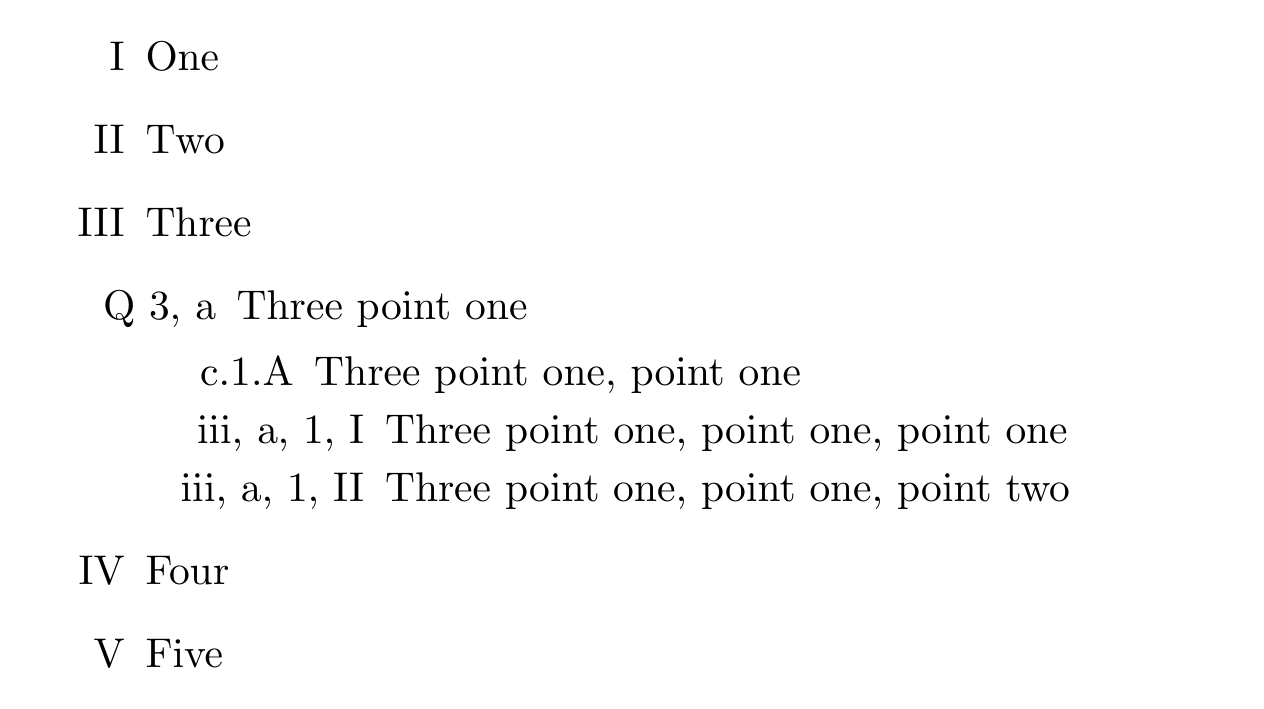
\includegraphics[width=8cm]{Examples/list_challenge.png}
        \captionsetup{justification=centering}
		\caption{List challenge}
        \end{figure}
	\end{block}
\end{frame}

\subsection{Tables}
\begin{frame}[fragile]{Tables}
    This segment explains how to use \LaTeX \xspace to create and customize tables: changing size/spacing, combining cells, applying colour to rows or cells, and so forth.
    We can start with one of the simplest examples of a table:
\begin{columns}
    \begin{column}{0.6 \textwidth}
    \begin{minted}[baselinestretch=1.2, fontsize=\footnotesize, style=pastie, escapeinside=|||,]{latex}
        
\documentclass{article} \usepackage[utf8]{inputenc}
\begin{document}
    \begin{center}
        \begin{tabular}{ c c c }
         cell1 & cell2 & cell3 \\ 
         cell4 & cell5 & cell6 \\  
         cell7 & cell8 & cell9    
        \end{tabular}
    \end{center}
\end{document}

        \end{minted}
		\end{column}
		\begin{column}{0.3 \textwidth}
        \begin{block}{Live!}
            Let's see the exact output of this code snippet \textcolor{latexBird}{live}!
        \end{block}
		\end{column}
    \end{columns}
    
The tabular environment is the default \LaTeX \xspace method to create tables. You must specify a parameter to this environment; here we use \{c c c\} which tells LaTeX that there are three columns and the text inside each one of them must be centred.
\end{frame}

\begin{frame}[fragile]{Tables with fixed length}
    When formatting a table you might require a fixed length either for each column or for the entire table. The following example adds the array package to document preamble: \mintinline{latex}{\usepackage{array}}.
\begin{columns}
    \begin{column}{0.6 \textwidth}
    \begin{minted}[baselinestretch=1.2, fontsize=\footnotesize, style=pastie, escapeinside=|||,]{latex}
        
\documentclass{article} \usepackage{array}
\begin{document}
    \begin{center} \begin{tabular}{ | m{5em} | m{1cm}| m{1cm} | } 
        \hline
        cell1 dummy text dummy text dummy text& cell2 & cell3 \\ 
        \hline
        cell1 dummy text dummy text dummy text & cell5 & cell6 \\ 
        \hline
        cell7 & cell8 & cell9 \\ \hline
    \end{tabular} \end{center}
\end{document}

        \end{minted}
		\end{column}
		\begin{column}{0.3 \textwidth}
        \begin{block}{Live!}
            Let's see the exact output of this code snippet \textcolor{latexBird}{live}!
        \end{block}
		\end{column}
    \end{columns}
    
In the tabular environment, the parameter m\{5em\} sets a length of 5em for first column (1cm for the other two) and centres the text in the middle of the cell.
\end{frame}

\begin{frame}[fragile]{Tables with fixed length - Continued}
    If you don't need to control the width of each cell, but of the entire table and then evenly distribute the space within, use the tabularx package: \mintinline{latex}{\usepackage{tabularx}}.
\begin{columns}
    \begin{column}{0.6 \textwidth}
    \begin{minted}[baselinestretch=1.2, fontsize=\footnotesize, style=pastie, escapeinside=|||,]{latex}
        
\documentclass{article} \usepackage{tabularx}
\begin{document}
    \begin{tabularx}{0.8\textwidth} { 
      | >{\raggedright\arraybackslash}X 
      | >{\centering\arraybackslash}X 
      | >{\raggedleft\arraybackslash}X | }
     \hline
     item 11 & item 12 & item 13 \\ \hline
     item 21  & item 22  & item 23  \\ \hline
    \end{tabularx}
\end{document}

        \end{minted}
		\end{column}
		\begin{column}{0.3 \textwidth}
        \begin{block}{Live!}
            Let's see the exact output of this code snippet \textcolor{latexBird}{live}!
        \end{block}
		\end{column}
    \end{columns}
The environment tabularx is more flexible. In the example the table width is set to 80\% of the document's text width. You can use any of the units to set this length.
The prefix inside braces sets the alignment of each column: the first to left, the second to center and the third to right.
\end{frame}

\begin{frame}[fragile]{Tables - Challenge}
    \begin{block}{Quiz}
        Try to recreate something like this: \\ \smallskip
        \begin{figure}
		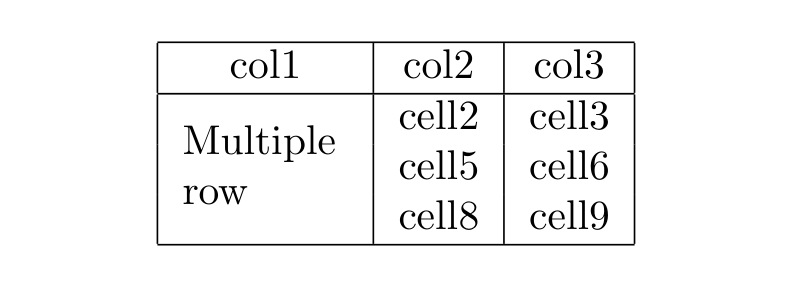
\includegraphics[width=8cm]{Examples/table_challenge.png}
        \captionsetup{justification=centering}
		\caption{Table challenge}
        \end{figure}
	\end{block}
\end{frame}

\begin{frame}[fragile]{Positioning tables}
    Positioning a table is easy if they're inside a float table environment.
\begin{columns}
    \begin{column}{0.6 \textwidth}
    \begin{minted}[baselinestretch=1.2, fontsize=\footnotesize, style=pastie, escapeinside=|||,]{latex}
        
\documentclass{article}
\begin{document}
    Below is a table positioned exactly here:
    \begin{table}[h!]
        \centering \begin{tabular}{||c c c c||} 
            \hline Col1 & Col2 & Col2 & Col3 \\ [0.5ex] 
            \hline \hline
            1 & 6 & 87837 & 787 \\ 
            2 & 7 & 78 & 5415 \\
            3 & 545 & 778 & 7507 \\
            4 & 545 & 18744 & 7560 \\
            5 & 88 & 788 & 6344 \\ [1ex] \hline
        \end{tabular}
    \end{table}
\end{document}

        \end{minted}
		\end{column}
		\begin{column}{0.3 \textwidth}
        \begin{block}{Live!}
            Let's see the exact output of this code snippet \textcolor{latexBird}{live}!
        \end{block}
		\end{column}
    \end{columns}
\end{frame}
\begin{frame}[fragile]{Positioning tables - Continued}
    The parameter h! establishes that this table must be placed here, and override \LaTeX \xspace defaults. The positioning parameters that can be passed-in include:
    \setbeamertemplate{itemize items}[circle]
    \begin{itemize}
        \item h: Will place the table here approximately.
        \item t: Position the table at the top of the page.
        \item b: Position the table at the bottom of the page.
        \item p: Put the table in a special page, for tables only.
        \item !: Override internal \LaTeX \xspace parameters.
        \item H: Place the table at this precise location, pretty much like h!.
        \item \mintinline{latex}{\centering} Centres the table relative to the float container element.
        \item 1ex: This adds extra space to the cell.
    \end{itemize}
\end{frame}

\begin{frame}[fragile]{Captions, labels and references of tables}
    Tables can be captioned, labelled and referenced by means of the table environment.
    \begin{columns}
    \begin{column}{0.6 \textwidth}
    \begin{minted}[baselinestretch=1.2, fontsize=\footnotesize, style=pastie, escapeinside=|||,]{latex}
        
\documentclass{article}
\begin{document}
    Table \ref{table:1} is an example of a referenced \LaTeX{} element.
    \begin{table}[h!]
        \centering \begin{tabular}{||c c c c||} 
            \hline Col1 & Col2 & Col2 & Col3 \\ [0.5ex] 
            \hline\hline
            1 & 6 & 87837 & 787 \\ 
            2 & 7 & 78 & 5415 \\
            3 & 545 & 778 & 7507 \\
            4 & 545 & 18744 & 7560 \\
            5 & 88 & 788 & 6344 \\ [1ex] \hline
        \end{tabular}
        \caption{Table to test captions and labels.} \label{table:1}
    \end{table}
\end{document}

        \end{minted}
		\end{column}
		\begin{column}{0.3 \textwidth}
        \begin{block}{Live!}
            Let's see the exact output of this code snippet \textcolor{latexBird}{live}!
        \end{block}
		\end{column}
    \end{columns}
\end{frame}

\begin{frame}[fragile]{Tables - Another challenge}
    \begin{block}{Quiz}
        Try to recreate something like this: \\ \smallskip
        \begin{figure}
		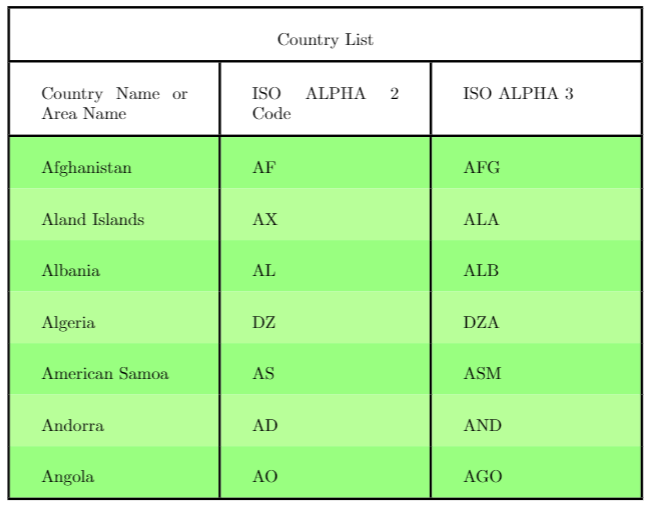
\includegraphics[width=6cm]{Examples/pos_table_challenge.png}
        \captionsetup{justification=centering}
		\caption{Colorful table challenge}
        \end{figure}
	\end{block}
\end{frame}


\subsection{Images}
\begin{frame}[fragile]{Images}
    \LaTeX \xspace can not manage images by itself, so we need to use the graphicx package. To use it, we include the following line in the preamble: \mintinline{latex}{\usepackage{graphicx}}.
    
    \begin{minted}[baselinestretch=1.2, fontsize=\footnotesize, style=pastie, escapeinside=|||,]{latex}
        
\documentclass{article} \usepackage{graphicx}
\graphicspath{ {./images/} }
\begin{document}
    The universe is immense and it seems to be homogeneous, 
    in a large scale, everywhere we look at.
    \includegraphics{universe.png}
    There's a picture of a galaxy above.
\end{document}

        \end{minted}
	  The command \mintinline{latex}{\graphicspath{ {./images/} }} tells \LaTeX \xspace that the images are kept in a folder named images under the directory of the main document.

    It is best practice to specify the graphics path to be relative to the main .tex file, denoting the main .tex file directory as ./ . The path can also be absolute.

\end{frame}

\begin{frame}[fragile]{Images - Continued}
    If we want to further specify how \LaTeX \xspace should include our image in the document (length, height, etc), we can pass those settings in the following format:

    \begin{minted}[baselinestretch=1.2, fontsize=\footnotesize, style=pastie, escapeinside=|||,]{latex}
        
\documentclass{article} \usepackage{graphicx}
\graphicspath{ {./images/} }
\begin{document}
    The universe is immense and it seems to be homogeneous, 
    in a large scale, everywhere we look at.
    \includegraphics[scale=1.5]{universe.png}
    \includegraphics[width=5cm, height=4cm]{universe.png}
    \includegraphics[width=\textwidth]{universe.png}
    \includegraphics[scale=1.2, angle=45]{universe.png}
    There's a picture of a galaxy above.
\end{document}

        \end{minted}
\end{frame}


\section{References and citations}
\begin{frame}[plain,noframenumbering]
    	\finalpage{\textcolor{Black}{\LARGE\textbf{References and citations}}}
    \end{frame}
\subsection{Hyperlinks}
\begin{frame}[fragile]{Hyperlinks}
    To make URL links and make the lines in the table of contents become links to the corresponding pages in the document, we simply add this line in the preamble of the document \mintinline{latex}{\usepackage{hyperref}}. \\
    
    \textcolor{red}{WARNING}: One must be careful when importing hyperref: usually, it has to be the last package to be imported—but there might be some exceptions to this rule. The reason is that it redefines many \LaTeX \xspace commands. It's a rule of thumb that helps to avoid errors.

\end{frame}

\begin{frame}[fragile]{\mintinline{latex}{URL} and \mintinline{latex}{href} command}
    Links to a web address or email can added to a \LaTeX \xspace file using the \mintinline{latex}{\url{LINK}} command to display the actual link or \mintinline{latex}{\href{LINK}{TEXT}} to use a hidden link and show a word/sentence instead.
    
    \begin{columns}
    \begin{column}{0.6 \textwidth}
    \begin{minted}[baselinestretch=1.2, fontsize=\footnotesize, style=pastie, escapeinside=|||,]{latex}
        
\documentclass{article} \usepackage{hyperref}
\begin{document}
    \url{https://google.com/}\\
    \href{https://google.com/}{Google}
\end{document}

        \end{minted}
		\end{column}
		\begin{column}{0.3 \textwidth}
        \begin{block}{Result}
           \url{https://google.com/}\\
    \href{https://google.com/}{Google}
        \end{block}
		\end{column}
    \end{columns}
\end{frame}

\begin{frame}[fragile]{Hyperlinks styles and colors}
    The default formatting for links can be changed so the information in your documents is more clearly presented. Below you can see an example:
    
    \begin{minted}[baselinestretch=1.2, fontsize=\footnotesize, style=pastie, escapeinside=|||,]{latex}
        
\documentclass{article} \usepackage{hyperref}
\hypersetup{
    colorlinks=true, linkcolor=blue,
    filecolor=magenta, urlcolor=cyan,
    pdftitle={Overleaf Example}, pdfpagemode=FullScreen,
}
\urlstyle{same}

\begin{document}
    ...
\end{document}

        \end{minted}
\end{frame}

\begin{frame}[fragile]{Hyperlinks styles and colors - Continued}
    \begin{description}
        \item[\mintinline{latex}{\hypersetup{ ... }}] This will set the options to configure the behaviour of the links within the document. Every parameter must be comma-separated and the syntax must be in the format parameter=value.
        \item[colorlinks=true] Links will be colored, the default color is red.
        \item[linkcolor=blue] Internal links are displayed in blue.
        \item[filecolor=magenta] Links to local files will be shown in magenta color.
        \item[urlcolor=cyan] Links to web sites are set to cyan color.
        \item[\mintinline{latex}{\urlstyle{same}}] Default settings print links in mono-style spaced fonts, this command changes that and displays the links in the same style as the rest of the text.
        \item[pdftitle={Overleaf Example}] Is the title of the PDF output file.
        \item[pdfpagemode=FullScreen] The document will be opened in full screen mode.
    \end{description}
\end{frame}

\begin{frame}[fragile]{Hyperlinks - Challenge}
    \begin{block}{Quiz}
        How to link local files?
	\end{block}
\end{frame}

\subsection{Bibliography}
\begin{frame}[fragile]{Bibliography: just a list of \mintinline{latex}{bibitems}}
    Bibliography and citation managment with \LaTeX \xspace is very easy.
    
    \LaTeX \xspace has a lot of packages for bibiliography. In this workshop, we use \hologo{BibTeX}:
    To use \hologo{BibTeX}
    \begin{enumerate}
        \item Create a database (.bib) file that describes the articles that you want to reference.
        \item Specify the style and location of the bibliography in your LaTeX document.
        \item Compile the file.
    \end{enumerate}
    You may ask why you should use \hologo{BibTeX}.
    \setbeamertemplate{itemize items}[circle]
    \setlength\itemsep{0.5mm}
    \begin{itemize}
        \item Let the style file worry about formatting the bibliography.
        \item Avoid retyping the same references for your different files and projects.
        \item It is more efficient.
    \end{itemize}

\end{frame}

\begin{frame}[fragile]{Bibliography - Example}
    The prototype of using \hologo{BibTeX} looks something like this:
        \begin{minted}[baselinestretch=1.2, fontsize=\footnotesize, style=pastie, escapeinside=|||,]{latex}
        
\documentclass{article}
\begin{document}
    ...
    \bibliographystyle{style}
    \bibliography{.bib file name}
\end{document}

        \end{minted}
We access bibitems with the \mintinline{latex}{\cite{NAME}} command. \\

For more information about \hologo{BibTeX} styles, look up \href{https://www.overleaf.com/learn/latex/Bibtex_bibliography_styles}{\color{latexBird}{\underline{this link}}}.\\

Let's see an example live.

\end{frame}

\section{Mathematical mode}
\begin{frame}[plain,noframenumbering]
    	\finalpage{\textcolor{Black}{\LARGE\textbf{Mathematical mode}}}
\end{frame}

\subsection{Mathematical expressions}
\begin{frame}[fragile]{Mathematical expressions}
    \LaTeX's features for typesetting mathematics make it a compelling choice for writing technical documents. This article shows the most basic commands needed to get started with writing maths using \LaTeX.\\
    Writing basic equations in LaTeX is straightforward, for example:
        \begin{minted}[baselinestretch=1.2, fontsize=\footnotesize, style=pastie, escapeinside=|||,]{latex}
        
\documentclass{article}
\begin{document}
    The well known Pythagorean theorem \(x^2 + y^2 = z^2\) was 
    proved to be invalid for other exponents. 
    Meaning the next equation has no integer solutions:
    \[ x^n + y^n = z^n \]
\end{document}

        \end{minted}
As you see, the way the equations are displayed depends on the delimiter, in this case \mintinline{latex}{\[...\]} and \mintinline{latex}{\(...\)}.
\end{frame}
\begin{frame}[fragile]{Mathematical expressions - Continued}
    \LaTeX \xspace allows two writing modes for mathematical expressions: the inline math mode and display math mode.
    \begin{description}
        \item[inline math mode] used to write formulas that are part of a paragraph.
        \item[display math mode] used to write expressions that are not part of a paragraph, and are therefore put on separate lines.
    \end{description}
\end{frame}
\begin{frame}[fragile]{Inline math mode}
    You can use any of these "delimiters" to typeset your math in inline mode: \\ \smallskip
    \hspace{5mm} $\blacksquare$ \mintinline{latex}{\(...\)} \\ \smallskip
    \hspace{5mm} $\blacksquare$ \mintinline{latex}{$...$} \\ \smallskip
    \hspace{5mm} $\blacksquare$ \mintinline{latex}{\begin{math}...\end{math}} \\
    They all work and the choice is a matter of taste, so let's see some examples.
        \begin{minted}[baselinestretch=1.2, fontsize=\footnotesize, style=pastie, escapeinside=|||,]{latex}
        
\documentclass{article} \begin{document}
    \noindent Writing inline by \verb|\(...\)|:
    \begin{quote} In physics, \(E=mc^2\), discovered in 1905 by Albert Einstein. \end{quote}
    
    \noindent Writing inline by \texttt{\$...\$}:
    \begin{quote} In physics, $E=mc^2$, discovered in 1905 by Albert Einstein. \end{quote}
    
    \noindent Writing inline by \verb|\begin{math}...\end{math}|:
    \begin{quote}\begin{math}E=mc^2\end{math}, discovered in 1905 by Albert Einstein. \end{quote}
\end{document}

        \end{minted}
\end{frame}
\begin{frame}[fragile]{Display math mode}
    You can use any of these "delimiters" to typeset your math in display mode: \\ \smallskip
    \hspace{5mm} $\blacksquare$ \mintinline{latex}{\[...\]} \\ \smallskip
    \hspace{5mm} $\blacksquare$ \mintinline{latex}{\begin{displaymath}...\end{displaymath}} \\ \smallskip
    \hspace{5mm} $\blacksquare$ \mintinline{latex}{\begin{equation}...\end{equation}} \\ \smallskip
    \hspace{5mm} $\blacksquare$ \mintinline{latex}{$$ ... $$} \\
    Display math mode has two versions which produce numbered or unnumbered equations. Let's look at a basic example:
        \begin{minted}[baselinestretch=1.2, fontsize=\footnotesize, style=pastie, escapeinside=|||,]{latex}
        
\documentclass{article} \begin{document}
    The mass-energy equivalence is described by the famous equation
    \[E=mc^2\]
    discovered in 1905 by Albert Einstein. 
    In natural units ($c$ = 1), the formula expresses the identity
    \begin{equation} E=m \end{equation}
\end{document}

        \end{minted}
\end{frame}
\begin{frame}[fragile]{Mathematical symbols}
Below is a table with some common maths symbols. For a more complete list see the \href{https://www.overleaf.com/learn/latex/List_of_Greek_letters_and_math_symbols}{\color{latexBird}{\underline{List of Greek letters and math symbols}}}:
    \begin{center}
        \scalebox{1}[1]{%
        \begin{tabular}{|c|l|l|l|}
                \hline
                \thead{\textbf{description}} &
                \thead{\textbf{code}} &
                \thead{\textbf{examples}} \\
                \hline
                
                Greek letters & \makecell[l]{\mintinline{latex}{\alpha \beta \gamma \rho \sigma \delta \epsilon}} & $ \alpha \beta \gamma \rho \sigma \delta \epsilon $ \\
                \hline
                
               Binary operators & \makecell[l]{\mintinline{latex}{\times \otimes \oplus \cup \cap}} & $\times \otimes \oplus \cup \cap $ \\
                \hline

                Relation operators & \makecell[l]{\mintinline{latex}{< > \subset \supset \subseteq \supseteq}} & $ < > \subset \supset \subseteq \supseteq $ \\
                \hline
                
                Others & \makecell[l]{\mintinline{latex}{\int \oint \sum \prod}} & $ \int \oint \sum \prod $ \\
                \hline

            \end{tabular}
        }
    \end{center}

\end{frame}

\subsection{Subscripts and superscripts}
\begin{frame}[fragile]{Subscripts and superscripts}
The symbols \_ and \^ are used for subscript and superscript respectively. can also be combined in the same expression, for example:

\begin{minted}[baselinestretch=1.2, fontsize=\footnotesize, style=pastie, escapeinside=|||,]{latex}
        
\documentclass{article} \begin{document}
    \[ \int\limits_0^1 x^2 + y^2 \ dx \]
    \[ \int_0^1 x^2 + y^2 \ dx \]
    \[ x^{2 \alpha} - 1 = y_{ij} + y_{ij}  \]
    \[ \sum_{i=1}^{\infty} \frac{1}{n^s} 
    = \prod_p \frac{1}{1 - p^{-s}} \]
\end{document}

        \end{minted}
\end{frame}
\subsection{Multiple integral}
\begin{frame}[fragile]{Multiple integral}
    To obtain double/triple/multiple integrals and cyclic integrals you must use amsmath and esint (for cyclic integrals) packages.

\begin{minted}[baselinestretch=1.2, fontsize=\footnotesize, style=pastie, escapeinside=|||,]{latex}
        
\documentclass{article} \usepackage{amsmath, esint}
\begin{document}
    \begin{gather*}
        \iint_V \mu(u,v) \,du\,dv
    \\
        \iiint_V \mu(u,v,w) \,du\,dv\,dw
    \\
        \iiiint_V \mu(t,u,v,w) \,dt\,du\,dv\,dw
    \\
        \idotsint_V \mu(u_1,\dots,u_k) \,du_1 \dots du_k
    \end{gather*}
\end{document}

        \end{minted}
\end{frame}


\subsection{Brackets and parentheses}
\begin{frame}[fragile]{Brackets and parentheses}
Parentheses and brackets are very common in mathematical formulas. You can easily control the size and style of brackets in \LaTeX. \\
Here's an table of listing some common math braces and parentheses used in \LaTeX. For more braces, look at \href{https://www.overleaf.com/learn/latex/Brackets_and_Parentheses}{\color{latexBird}{\underline{this link.}}} 
    \begin{center}
        \scalebox{1}[1]{%
        \begin{tabular}{|l|l|l|}
                \hline
                \thead{\textbf{Type}} &
                \thead{\textbf{\LaTeX \xspace markup}} &
                \thead{\textbf{Renders as}} \\
                \hline
                
                Parentheses; round brackets & \makecell[l]{\mintinline{latex}{(x+y)}} & $ (x+y) $ \\
                \hline
                
               Brackets; square brackets & \makecell[l]{\mintinline{latex}{[x+y]}} & $[x+y] $ \\
                \hline

                Braces; curly brackets & \makecell[l]{\mintinline{latex}{\{ x+y \}}} & $ \{ x+y \} $ \\
                \hline
                
                Angle brackets & \makecell[l]{\mintinline{latex}{\langle x+y \rangle}} & $ \langle x+y \rangle $ \\
                \hline
                
                Pipes; vertical bars & \makecell[l]{\mintinline{latex}{|x+y|}} & $ |x+y| $ \\
                \hline
                
                Double pipes & \makecell[l]{\mintinline{latex}{\|x+y\|}} & $ \|x+y\| $ \\
                \hline
            \end{tabular}
        }
    \end{center}
    The size of brackets and parentheses can be manually set, or they can be resized dynamically in your document, as shown in the next example:\\
    \mintinline{latex}{\[ 
 \left[  \frac{ N } { \left( \frac{L}{p} \right)  - (m+n) }  \right]
\]
}

\end{frame}

\subsection{Matrices}
\begin{frame}[fragile]{Matrices}
The \textsl{amsmath} package provides commands to typeset matrices with different delimiters. Once you have loaded amsmath in your preamble, you can use the following environments in your math environments:

    \begin{center}
        \scalebox{0.9}[0.9]{%
        \begin{tabular}{|l|l|c|}
                \hline
                \thead{\textbf{Type}} &
                \thead{\textbf{\LaTeX \xspace markup}} &
                \thead{\textbf{Renders as}} \\
                \hline
                
                Plain & 
                \makecell[l]{
                \mintinline{latex}{\begin{matrix} ... \end{matrix}}}& 
                $ \begin{matrix} 1 & 2 & 3 \\ a & b & c \end{matrix} $ \\
                \hline
                
               Parentheses; round brackets	 & 
                \makecell[l]{
                \mintinline{latex}{\begin{pmatrix} ... \end{pmatrix}}}& 
                $ \begin{pmatrix} 1 & 2 & 3 \\ a & b & c \end{pmatrix} $ \\
                \hline
                Brackets;
square brackets	 & 
                \makecell[l]{
                \mintinline{latex}{\begin{bmatrix} ... \end{bmatrix}}}& 
                $ \begin{bmatrix} 1 & 2 & 3 \\ a & b & c \end{bmatrix} $ \\
                \hline
                Braces;
curly brackets & 
                \makecell[l]{
                \mintinline{latex}{\begin{Bmatrix} ... \end{Bmatrix}}}& 
                $ \begin{Bmatrix} 1 & 2 & 3 \\ a & b & c \end{Bmatrix} $ \\
                \hline
                Pipes	 & 
                \makecell[l]{
                \mintinline{latex}{\begin{vmatrix} ... \end{vmatrix}}}& 
                $ \begin{vmatrix} 1 & 2 & 3 \\ a & b & c \end{vmatrix} $ \\
                \hline
                Double pipes & 
                \makecell[l]{
                \mintinline{latex}{\begin{Vmatrix} ... \end{Vmatrix}}}& 
                $ \begin{Vmatrix} 1 & 2 & 3 \\ a & b & c \end{Vmatrix} $ \\
                \hline
            \end{tabular}
        }
    \end{center}

\end{frame}
\begin{frame}[fragile]{Matrices - Challenge}
    \begin{block}{Quiz}
        Create something like this:
        $$
        \left\langle
        \begin{matrix}
        1 & 2 & 3\\
        a & b & c
        \end{matrix}
        \right\rvert	
        $$
	\end{block}
\end{frame}

\subsection{Fractions}
\begin{frame}[fragile]{Fractions}
Using fractions and binomial coefficients in an expression is straightforward.
For these commands to work you must import the package amsmath by adding the next line to the preamble of your file
    \begin{minted}[baselinestretch=1.2, fontsize=\footnotesize, style=pastie, escapeinside=|||,]{latex}
        
\documentclass{article} \begin{document}
    The binomial coefficient is defined by the next expression:
    \[
        \binom{n}{k} = \frac{n!}{k!(n-k)!}
    \]
\end{document}

        \end{minted}
\end{frame}

\begin{frame}[fragile]{Continued fractions}
The usage of fractions is quite flexible, they can be nested to obtain more complex expressions.

    \begin{minted}[baselinestretch=1.2, fontsize=\footnotesize, style=pastie, escapeinside=|||,]{latex}
        
\documentclass{article} \begin{document}
    The fractions can be nested
    \[ \frac{1+\frac{a}{b}}{1+\frac{1}{1+\frac{1}{a}}} \]
    
    Now a wild example
    \[
      a_0+\cfrac{1}{a_1+\cfrac{1}{a_2+\cfrac{1}{a_3+\cdots}}}
    \]
\end{document}

        \end{minted}
\mintinline{latex}{\cfrac} command displays nested fractions without changing the size of the font. Specially useful for continued fractions.
\end{frame}

\subsection{Aligning equations}
\begin{frame}[fragile]{Aligning equations}
The amsmath package provides a handful of options for displaying equations. You can choose the layout that better suits your document, even if the equations are really long, or if you have to include several equations in the same line.

The standard LaTeX tools for equations may lack some flexibility, causing overlapping or even trimming part of the equation when it's too long. We can surpass such difficulties by using the amsmath package.


    \begin{minted}[baselinestretch=1.2, fontsize=\footnotesize, style=pastie, escapeinside=|||,]{latex}
        
\documentclass{article} \begin{document}
    \begin{equation} \label{eq1}
        \begin{split}
            A & = \frac{\pi r^2}{2} \\
              & = \frac{1}{2} \pi r^2
        \end{split}
    \end{equation}
\end{document}

        \end{minted}
\end{frame}

\begin{frame}[fragile]{Displaying long equations}
For equations longer than a line use the \textsl{multline} environment. Insert a double backslash to set a point for the equation to be broken. The first part will be aligned to the left and the second part will be displayed in the next line and aligned to the right.


The standard LaTeX tools for equations may lack some flexibility, causing overlapping or even trimming part of the equation when it's too long. We can surpass such difficulties by using the amsmath package.


    \begin{minted}[baselinestretch=1.2, fontsize=\footnotesize, style=pastie, escapeinside=|||,]{latex}
        
\documentclass{article} \begin{document}
    \begin{multline*}
        p(x) = 3x^6 + 14x^5y + 590x^4y^2 + 19x^3y^3 \\ 
        - 12x^2y^4 - 12xy^5 + 2y^6 - a^3b^3
    \end{multline*}
\end{document}

        \end{minted}
    \textsl{Split} is very similar to \textsl{multline}.
\end{frame}

\begin{frame}[fragile]{Aligning several equations}
If there are several equations that you need to \textsl{align} vertically, the align environment will do it:
    \begin{minted}[baselinestretch=1.2, fontsize=\footnotesize, style=pastie, escapeinside=|||,]{latex}
        
\documentclass{article} \begin{document}
    \begin{align*}
        x&=y           &  w &=z              &  a&=b+c \\
        2x&=-y         &  3w&=\frac{1}{2}z   &  a&=b \\
        -4 + 5x&=2+y   &  w+2&=-1+w          &  ab&=cb
    \end{align*}
\end{document}

        \end{minted}
\end{frame}

\begin{frame}[fragile]{Grouping and centering equations}
If you just need to display a set of consecutive equations, centered and with no alignment whatsoever, use the \textsl{gather} environment. The asterisk trick to set/unset the numbering of equations also works here.

    \begin{minted}[baselinestretch=1.2, fontsize=\footnotesize, style=pastie, escapeinside=|||,]{latex}
        
\documentclass{article} \begin{document}
    \begin{gather*} 
        2x - 5y =  8 \\ 
        3x^2 + 9y =  3a + c
    \end{gather*}
\end{document}

        \end{minted}
\end{frame}


\begin{frame}[fragile]{Aligning - Challenge}
    \begin{block}{Quiz}
        Create something like this:
    $$Constraints:$$
    $$ \frac{1}{6000} \, y_1 + \frac{1}{5000} \, y_2 + \frac{10}{3000} \, y_3 \leq 5 $$
    $$ \frac{40}{1000} \, y_1 + \frac{45}{1000} \, y_2 + \frac{210}{1000} \, y_3 \leq 6,000 $$
    \begin{align*} \begin{split}
        5,000 \leq \, & y_1 \leq\, 10,000 \\
        & y_2 \leq \, 15,000 \\
        4,000 \leq \, & y_3 \leq\, 8,000
    \end{split} \end{align*}
    $$\forall i \in \{\,1,\,2,\,3\,\} \Rightarrow y_i \in \mathbb Z^+_0$$
    $$Objective: Maximize \,\,\, 4 \, y_1 + 6 \, y_2 + 10 \, y_3.$$

	\end{block}
\end{frame}

\subsection{Spacing in math mode}
\begin{frame}[fragile]{Spacing in math mode}
The example below contains a complete list of spaces inserted using various commands and demonstrates their effect on the typeset math.


    \begin{minted}[baselinestretch=1.2, fontsize=\footnotesize, style=pastie, escapeinside=|||,]{latex}
        
\documentclass{article} \usepackage{amsmath}
\begin{document}
    Spaces in mathematical mode.
    \begin{align*}
        f(x) &= x^2\! +3x\! +2 \\
        f(x) &= x^2+3x+2 \\
        f(x) &= x^2\, +3x\, +2 \\
        f(x) &= x^2\: +3x\: +2 \\
        f(x) &= x^2\; +3x\; +2 \\
        f(x) &= x^2\ +3x\ +2 \\
        f(x) &= x^2\quad +3x\quad +2 \\
        f(x) &= x^2\qquad +3x\qquad +2
    \end{align*}
\end{document}

        \end{minted}
\end{frame}

\begin{frame}[fragile]{Spacing in math mode - Continued}
    Here's description of spacing commands:
    \begin{center}
        \scalebox{1}[1]{%
        \begin{tabular}{|c|l|}
                \hline
                \thead{\textbf{\LaTeX \xspace code}} & 
                \thead{\textbf{Description}}  \\
                \hline
                
                \mintinline{latex}{\quad} & \makecell[l]{space equal to the current font size (= 18 mu)} \\
                \hline
                
                \mintinline{latex}{\,} & \makecell[l]{3/18 of quad (= 3 mu)} \\
                \hline

                \mintinline{latex}{\:} & \makecell[l]{4/18 of quad (= 4 mu)} \\
                \hline
                
                \mintinline{latex}{\;} & \makecell[l]{5/18 of quad (= 5 mu)} \\
                \hline
                
                \mintinline{latex}{\!} & \makecell[l]{-3/18 of quad (= -3 mu).} \\
                \hline
                
                \mintinline{latex}{\ (space after backslash!)} & \makecell[l]{equivalent of space in normal text} \\
                \hline
                
                \mintinline{latex}{\qquad} & \makecell[l]{twice of quad (= 36 mu)} \\
                \hline
            \end{tabular}
        }
    \end{center}

\end{frame}

%\section{References}
%\begin{frame}[plain,noframenumbering]
%    \finalpage{\textcolor{Black}{\LARGE\textbf{References}}}
%\end{frame}

%\begin{frame}[allowframebreaks]{References}
%		\nocite{*}
%		\bibliographystyle{unsrt}
%		\bibliography{Bibliography}
%\end{frame}
\end{document} 